\documentclass[11pt]{article}
\usepackage[T1]{fontenc}
\usepackage{lmodern}
\input{glyphtounicode-cmex}
\usepackage{amsmath,amssymb,amsthm,mathtools}
\usepackage[margin=1in]{geometry}
\usepackage{microtype}
\usepackage{booktabs}
\usepackage{tikz}
\usetikzlibrary{arrows.meta,positioning,calc,fit}
\usepackage{xcolor}
\usepackage{url}
\usepackage[colorlinks=true,linkcolor=blue!45!black,citecolor=blue!45!black,
  urlcolor=blue!45!black,pdfauthor={OpenAI},
  pdftitle={A power saving for intersective polynomial differences with an exponent depending only on the degree}]{hyperref}

\newtheorem{theorem}{Theorem}[section]
\newtheorem{proposition}[theorem]{Proposition}
\newtheorem{lemma}[theorem]{Lemma}
\newtheorem{corollary}[theorem]{Corollary}
\theoremstyle{definition}
\newtheorem{definition}[theorem]{Definition}
\theoremstyle{remark}
\newtheorem{remark}[theorem]{Remark}
\numberwithin{equation}{section}
\newcommand{\N}{\mathbb N}
\newcommand{\Z}{\mathbb Z}
\newcommand{\Q}{\mathbb Q}
\newcommand{\R}{\mathbb R}
\newcommand{\C}{\mathbb C}
\newcommand{\F}{\mathbb F}
\newcommand{\E}{\mathbb E}
\newcommand{\1}{\mathbf 1}
\newcommand{\eps}{\varepsilon}
\newcommand{\abs}[1]{\lvert#1\rvert}
\newcommand{\norm}[1]{\lVert#1\rVert}
\DeclareMathOperator{\supp}{supp}
\DeclareMathOperator{\rad}{rad}
\DeclareMathOperator{\id}{id}
\newcommand{\articleid}[1]{\nolinkurl{#1}}
\allowdisplaybreaks[1]

\title{A power saving for intersective polynomial differences\\
with an exponent depending only on the degree}
\author{OpenAI}
\date{October 5, 2026}

\begin{document}
\maketitle
\begin{abstract}
An integer polynomial is intersective if it has a root modulo every positive
integer. For each degree $k\ge2$, we prove that there is an exponent $c_k>0$
such that every set $A\subseteq\{1,\ldots,N\}$ whose differences avoid all nonzero values $h(1),h(2),\ldots$,
where $h$ is an intersective polynomial of degree $k$ with positive leading
coefficient, satisfies
$|A|=O_h(N^{1-c_k})$. The implied constant may depend on $h$, but the
power-saving exponent depends only on its degree.
\end{abstract}

\tableofcontents

\section{Introduction}\label{sec:introduction}

For a polynomial $h\in\Z[x]$, consider how large a set of integers can be
if no difference between two of its elements is a nonzero value of $h$.
Write $\N_+=\{1,2,\ldots\}$, $[N]=\{1,\ldots,N\}$, and
$A-A=\{a-b:a,b\in A\}$. We call $h$ \emph{intersective} if, for every
integer $q\ge1$, some integer $t$ satisfies $h(t)\equiv0\pmod q$.
This is the necessary local condition for polynomial differences in every
set of positive density: if $h$ has no root modulo $q$, the multiples of
$q$ contain no difference in $h(\N_+)$. The condition allows the roots at
different moduli to arise from different factors of $h$; a rational root is
not required.

\begin{theorem}\label{thm:main}
For every integer $k\ge2$, there is a constant $c_k\in(0,1)$ with the
following property. For every intersective polynomial $h\in\Z[x]$ of degree
$k$ with positive leading coefficient, there are a constant $C_h\ge1$ and an
integer $N_h\ge1$ such that, whenever $N\ge N_h$ and $A\subseteq[N]$ satisfy
\[
 (A-A)\cap h(\N_+)\subseteq\{0\},
\]
one has
\[
 |A|\le C_h N^{1-c_k}.
\]
\end{theorem}

The exponent is common to all polynomials of a fixed degree. The constants
$C_h,N_h$ may depend on every coefficient of $h$, and $h$ remains fixed as
$N$ grows. The theorem concerns ordinary integer differences; zero values of
$h$ impose no restriction on $A$.

\subsection{History and relation to earlier work}

Furstenberg~\cite{Furstenberg1977} and S\'ark\"ozy~\cite{Sarkozy1978}
proved that every set of positive upper density contains two elements
whose difference is a nonzero square. Their proofs introduced distinct
ergodic and Fourier-analytic approaches to this recurrence problem.
Kamae and Mend\`es France~\cite{KamaeMendesFrance1978} extended the
positive-density conclusion to nonconstant intersective polynomials. Together with
the elementary congruence obstruction above, this identifies the exact
class of nonconstant polynomials for which the density of an avoiding set must tend
to zero.

The quantitative problem has driven successive refinements of Fourier
density-increment methods. For square differences, Pintz, Steiger, and
Szemer\'edi~\cite{PintzSteigerSzemeredi1988} introduced a substantially
stronger iteration. Bloom and Maynard~\cite{BloomMaynard2022} later
obtained the bound
\[
 |A|\ll N(\log N)^{-c\log\log\log N}
\]
using estimates for the additive energy of rational numbers.
For general intersective polynomials, Lucier~\cite{Lucier2006} established
quantitative bounds using auxiliary polynomials adapted to progressions,
and Rice~\cite{Rice2019} developed stronger estimates by combining
iteration with sieved polynomial sums.
Arala~\cite{Arala2024} extended the Bloom--Maynard bound to every
intersective polynomial of degree at least two, with a constant depending
only on the degree in the exponent of $\log N$.

Green and Sawhney~\cite[Theorem~1.1]{GreenSawhney2025} obtained the
square-difference bound
\[
 |A|\ll N\exp(-c\sqrt{\log N}).
\]
Their arithmetic
level-$d$ inequality and random sparsification also underpin the recent
general-polynomial result of Adajar et al.~\cite[Theorem~1.1]{AdajarEtAl2026}:
for every fixed intersective $h$ of degree at least two and every fixed
$0<\mu<1/2$,
\[
 |A|\le N\exp\bigl(-c_{h,\mu}(\log N)^\mu\bigr)
\]
for sufficiently large $N$. Theorem~\ref{thm:main} gives a fixed power
of $N$ as the saving, with an exponent common to all polynomials of each
fixed degree.

The immediate predecessor for our method is the power-saving theorem
for square differences in~\cite[Theorem~1.1]{squarepower}. Its proof
uses finite reflection-positive tuple laws and a signed multilinear
functional. Hatami~\cite{Hatami2010} gave a multilinear H\"older criterion
for graph norms. Reflection and Cauchy--Schwarz arguments are central to
the reflection-group constructions of Conlon and Lee~\cite{ConlonLee2017}.
Here we adapt the specific laws and functional of~\cite{squarepower},
with all required proofs included, and supply the polynomial and
change-of-scale arguments described next.

\subsection{The argument and its principal constructions}

The square-difference method constructs a multilinear form
which dominates a fixed power of density, and proves that this form contracts
on passing to shorter intervals. We retain this organization, but polynomial
values require two additional compatibilities: the polynomial changes when
one passes to a progression, and the local distribution supplied by the
multilinear construction need not be the natural distribution of polynomial
values.

\paragraph{Normalizing the local coefficients.}
We first pass from the polynomial in Theorem~\ref{thm:main} to a polynomial
$g(x)=h(r+D_0x)/M$ for which the first nonzero Taylor coefficient at one
chosen root in each $\Z_p$ is a unit. Only finitely many primes require the
extra division by $M$. The multiplicity of each chosen root is retained, and
the representative $r$ is chosen so that positive inputs for $g$ give positive
inputs for $h$. The purpose is to make the local numerical choices that
determine the final exponent depend only on the degree.

\paragraph{A family closed under passage to progressions.}
Section~\ref{sec:local} retains the auxiliary construction for an arbitrary
fixed intersective polynomial $h$. It gives integer polynomials $h_l$, indexed by
$l\in\N_+$, with $h_1=h$, and a fixed completely multiplicative function
$\lambda:\N_+\to\N_+$ such that, for all positive integers $l,D$,
\[
 h_l(Dx-i)=\lambda(D)h_{lD}(x)
 \quad\text{for some }0\le i<D,
 \qquad D\mid\lambda(D),\quad \lambda(D)\le D^{\deg h}.
\]
Consequently, a subset of an arithmetic progression of step $\lambda(D)$
which avoids nonzero $h_l$-differences becomes, in progression coordinates,
a set avoiding nonzero $h_{lD}$-differences. Compatible roots in the rings
$\Z_p$ produce the family. Its coefficient bounds, complete exponential-sum
estimates, and local lifting properties are uniform in $l$.

Applied to $g$, the family retains the zero valuation of the first nonzero
coefficient at each chosen root: Lucier's auxiliary formula preserves that
valuation \cite[Section~8]{Lucier2006}. Thus every auxiliary polynomial for
$g$ is nonconstant as an element of $\F_p[x]$ for every prime $p$. For
$p>k$, its reduced derivative is nonzero, and the complete-sum estimates hold
beyond a threshold depending only on $k$. At the finitely many smaller primes below that
threshold, interpolation bounds the derivative valuation at some argument in
terms of $k$ and $p$. These bounds make the lifting moduli and cycle length,
and hence the number of tuple slots below, depend only on $k$.

\paragraph{Weighted forms that follow the family.}
For each sufficiently large prime $p$, Section~\ref{sec:tuples} constructs a
probability distribution on tuples $(z_v)_{v\in V}\in\F_p^V$, where $V$ is
one fixed finite set of even cardinality $d$. A distinguished cycle of slots
has increments among the values of $h_l$ at arguments where its derivative is
nonzero modulo $p$, apart from a small exceptional part of the distribution.
The constraint on an edge is weighted by the number of such arguments giving
its increment. This weight has a Fourier bound uniform in the auxiliary
polynomial and transforms exactly under the progression identity above.

The laws are reflection positive: the quadratic form obtained by splitting
the slots across any of a specified family of reflections is positive
semidefinite. They also have uniform individual marginals and a conditional
mixing estimate. Section~\ref{sec:lifts} derives the resulting signed
H\"older inequality and estimates for Fourier lifts. At scale $N$, the lift
retains the normalized Fourier coefficients of $1_A$ at rational frequencies
whose denominators are at most a small fixed power of $N$. Integrating its
product over the $d$ slots gives a nonnegative quantity $Y_l(N,A)$ satisfying
\[
 Y_l(N,A)\ge (|A|/N)^d.
\]
The associated seminorm permits comparison along progressions with a factor
tending to one, rather than a fixed loss at every scale.

\paragraph{A kernel realizing the resulting increment distribution.}
The increment distribution of two slots is determined by the whole tuple
construction. It is supported on regular polynomial values, but there is no
reason for it to equal the distribution obtained by evaluating $h_l$ at a
uniform argument. Section~\ref{sec:kernel} constructs a signed kernel on
actual positive values of $h_l$ whose Fourier transform approximates the
desired local multipliers. At each sufficiently large prime, a density on regular arguments
realizes the prescribed increment distribution. A truncated divisor
expansion combines these densities, while uniform lifting handles
characters of higher prime-power conductor. Minor arcs are controlled by
elementary Weyl differencing.

Only support is needed to use this kernel: its bilinear form vanishes on two
ordered subsets of an avoiding set, regardless of the signs of the kernel
weights. Its Fourier approximation therefore gives cancellation for the
chosen pair of slots. This separates the construction of a useful tuple law
from the problem of realizing its pair distribution on integer polynomial
values.

\paragraph{Contraction while the auxiliary parameter grows.}
Section~\ref{sec:transfer} combines the kernel estimate with the seminorm
comparison. A fixed positive proportion of assignments of residue classes
at the finitely many small primes gives cancellation. The other assignments,
together with the summable exceptional parts of the tuple laws, are bounded
using shorter intervals and polynomials farther along the family.
Section~\ref{sec:induction} closes the resulting recurrence with a bound
that holds for some fixed $a,b>0$, simultaneously for every $l$ and every set $A$
avoiding nonzero $h_l$-differences:
\[
 Y_l(N,A)\le C l^bN^{-a}.
\]
The factor $l^b$ is necessary to accommodate the
growth of the auxiliary polynomial: when $l$ is large relative to $N$, a
uniform subpower bound suffices, while the kernel supplies contraction in
the remaining range. For the normalized polynomial $g$, the parameters can
be chosen so that $a/d$ depends only on $k$. Taking $l=1$ and using density
domination bounds sets avoiding nonzero $g$-differences. Partitioning $A$
into residue classes modulo $M$, and using $Mg(n)=h(r+D_0n)$ with
$r+D_0n\ge1$, then transfers the bound to $h$ and proves
Theorem~\ref{thm:main}.

The polynomial argument thus adds exact covariance of the weighted tuple laws
across the auxiliary family and a signed polynomial kernel realizing their
pair multipliers. The initial normalization controls the structural parameters
that determine the exponent. All the estimates needed from the
reflection-positive method are proved below.

\subsection{Notation and uniformity}

We write $e(x)=\exp(2\pi i x)$ and use the negative sign in Fourier
coefficients. For $\xi\in\Q/\Z$, let $q(\xi)$ be its reduced positive
denominator, with $q(0)=1$. Averages, measures, and norms on finite sets use
uniform probability measure unless a different measure is specified.
For a positive integer $n$, write $\rad(n)=\prod_{p\mid n}p$, with
$\rad(1)=1$.
Empty products equal $1$, and a product space with no coordinates is a
singleton. Conditional expectations are with respect to the law specified
in the surrounding statement.

The auxiliary-family development applies to any fixed intersective polynomial
$h$ with chosen roots, and we write $k=\deg h$. Constants in $O(\cdot)$ and
$\ll$ may depend on this fixed datum and on parameters already fixed from it;
they are independent of the varying integers, sets, and auxiliary index $l$,
unless a restriction is explicitly stated. Likewise, sufficiently-large
thresholds are uniform in those varying data. We explicitly identify the
structural choices that depend only on $k$ when the first nonzero coefficient
at every chosen root is a unit. Bounds denoted $O_k(\cdot)$ are uniform over
all fixed data of degree $k$ satisfying those choices. A bound $N^{o(1)}$
means $C_\epsilon N^\epsilon$ for every $\epsilon>0$ under the same
uniformity convention. All structural parameters are fixed before the
asymptotic scale $N$ varies.

\section{Auxiliary polynomials and local estimates}\label{sec:local}

Passing to an arithmetic progression changes the polynomial whose values are
forbidden differences. We first show that one such change can make the first
nonzero Taylor coefficient at each chosen local root a unit. We then organize
all subsequent changes into a coherent family \(h_l\), indexed by positive
integers, and show that this local property is preserved. The family and its
local estimates remain available for an arbitrary fixed intersective
polynomial; the unit condition will let us choose their structural parameters
using only the degree. The estimates give decay of complete exponential sums
at large primes, together with residue classes on which polynomial values
lift uniformly and support cycles of one fixed length.

Throughout this section, \(h\in\Z[x]\) is the fixed intersective polynomial of
degree \(k\ge2\), with positive leading coefficient \(a\).

\subsection{A family compatible with progressions}

We use Lucier's auxiliary-polynomial construction
\cite[Section~8]{Lucier2006}, in which a compatible root at each prime
determines the normalization by its multiplicity. We give the construction
and its inheritance rule explicitly, before proving the uniform local
estimates needed here.

Here \(\Z_p\) denotes the ring of compatible residues modulo the powers of
a prime \(p\), and \(v_p\) its valuation, with \(v_p(0)=\infty\).
Every nonzero element is a power of \(p\) times a unit, so \(\Z_p\) is an
integral domain. Intersectivity supplies a root of \(h\) modulo every power
of \(p\). These roots can be chosen compatibly: at each stage, retain a
residue class having root extensions to arbitrarily high powers, and then
choose one of its finitely many refinements with the same property. Fix the
resulting root \(\mathfrak z_p\in\Z_p\) for each prime \(p\), and write
\[
 h(\mathfrak z_p+X)=\sum_{j=m_p}^k b_{j,p}X^j,
 \qquad 1\le m_p\le k,
 \qquad b_{m_p,p}\ne0.
\]
Thus \(m_p\) is the multiplicity of the chosen root.

The coefficient \(b_{m_p,p}\) is a unit for all sufficiently large primes,
with a threshold depending only on \(h\). To see this, factor
\(h=c\prod_i g_i^{d_i}\), where \(c\) is a nonzero integer and the \(g_i\)
are pairwise nonassociate primitive irreducible polynomials in \(\Z[x]\). Cleared
B\'ezout identities for \((g_i,g_j)\), \(i\ne j\), and for \((g_i,g_i')\)
have nonzero integer right-hand sides. Exactly one factor \(g_i\) vanishes
at \(\mathfrak z_p\), and \(g_i'(\mathfrak z_p)\ne0\). Outside the finite
set of primes dividing these right-hand sides or \(c\), the derivative and
all other factor values at \(\mathfrak z_p\) are units. Hence \(m_p=d_i\)
and
\[
 b_{m_p,p}
 =c\,g_i'(\mathfrak z_p)^{d_i}
       \prod_{j\ne i}g_j(\mathfrak z_p)^{d_j}
\]
is a unit. This argument allows repeated factors of \(h\).

We will sometimes impose the following additional condition on the chosen
roots:
\begin{equation*}\tag{U}\label{local:unit-condition}
 b_{m_p,p}\in\Z_p^\times\qquad\text{for every prime }p.
\end{equation*}
The construction below works without this condition. Its role is to make the
local parameter choices depend only on \(k\). Every intersective polynomial
can be reduced to this case by one progression change.

\begin{lemma}[Normalization at the chosen roots]\label{local:normalization}
There are positive integers \(D_0,M\), an integer \(-D_0<r\le0\), and an
intersective polynomial
\[
 g(x)=\frac{h(r+D_0x)}{M}\in\Z[x]
\]
of degree \(k\) with positive leading coefficient such that, for every prime
\(p\), the element \(w_p=(\mathfrak z_p-r)/D_0\) belongs to \(\Z_p\) and
\[
 g(w_p+X)=\sum_{j=m_p}^k b^*_{j,p}X^j,
 \qquad b^*_{j,p}\in\Z_p,
 \qquad b^*_{m_p,p}\in\Z_p^\times.
\]
Thus \(g\), with these chosen roots, satisfies
Condition~\eqref{local:unit-condition}. Moreover, for every \(n\in\N_+\),
\[
 Mg(n)=h(r+D_0n),\qquad r+D_0n\ge1.
\]
\end{lemma}

\begin{proof}
Put \(u'_p=v_p(b_{m_p,p})\). These are nonnegative integers, and the
factorization argument above shows that
\(S_0=\{p:u'_p>0\}\) is finite. For \(p\in S_0\), take
\(u_p=u'_p+1\), and set
\[
 D_0=\prod_{p\in S_0}p^{u_p},
 \qquad M=\prod_{p\in S_0}p^{u_pm_p+u'_p}.
\]
Choose the representative \(-D_0<r\le0\) satisfying
\(r\equiv\mathfrak z_p\pmod{p^{u_p}}\) for every \(p\in S_0\), by the
Chinese remainder theorem. If \(S_0\) is empty, these definitions give
\(D_0=M=1\) and \(r=0\).

For \(p\in S_0\), the congruence defining \(r\) shows that
\(w_p=(\mathfrak z_p-r)/D_0\) lies in \(\Z_p\); for \(p\notin S_0\), the
same conclusion follows because \(D_0\) is a \(p\)-adic unit. Define \(g\)
initially as the displayed rational polynomial. Its centered expansion is
\[
 g(w_p+X)=\sum_{j=m_p}^k b_{j,p}\frac{D_0^j}{M}X^j.
\]
If \(p\in S_0\), the coefficient at \(j=m_p\) has valuation
\(u'_p+u_pm_p-(u_pm_p+u'_p)=0\). For \(j>m_p\), its valuation is at least
\[
 u_p(j-m_p)-u'_p\ge1.
\]
If \(p\notin S_0\), both \(D_0\) and \(M\) are \(p\)-adic units, so every
coefficient is integral and the coefficient at \(j=m_p\) is again a unit.
Thus the centered expansion belongs to \(\Z_p[X]\) for every prime \(p\).
Translation by \(-w_p\in\Z_p\) shows that \(g\) itself belongs to
\(\Z_p[x]\). Every rational coefficient of \(g\) is therefore integral at
every prime and hence is an integer.

The elements \(w_p\) are roots of \(g\); reducing them at the prime-power
factors of any modulus and applying the Chinese remainder theorem proves
intersectivity. The degree and sign of the leading coefficient are preserved
because \(D_0,M>0\). Finally, the defining identity for \(g\) gives
\(Mg(n)=h(r+D_0n)\), and \(r>-D_0\) gives \(r+D_0n\ge1\) for \(n\ge1\).
\end{proof}

In the coordinates of any progression of step \(M\), a nonzero difference
\(g(n)\), \(n\ge1\), therefore gives the nonzero original difference
\(h(r+D_0n)\) at a positive argument. This will transfer the final bound for
\(g\) back to the original polynomial. We continue below with the arbitrary
fixed polynomial \(h\) and its chosen roots, assuming
Condition~\eqref{local:unit-condition} only when explicitly stated.

Define a completely multiplicative function \(\lambda:\N_+\to\N_+\) by
\(\lambda(p)=p^{m_p}\). For each \(l\ge1\), let \(r_l\) be the unique
integer in \((-l,0]\) satisfying
\[
 r_l\equiv\mathfrak z_p\pmod{p^{v_p(l)}}
 \qquad(p\mid l),
\]
and set
\[
 h_l(x)=\frac{h(r_l+lx)}{\lambda(l)},
 \qquad a_l=\frac{a l^k}{\lambda(l)}.
\]
For \(l=1\), this convention gives \(r_1=0\) and \(h_1=h\).

\begin{lemma}[The auxiliary family]\label{local:family}
For every \(l\ge1\), the polynomial \(h_l\) belongs to \(\Z[x]\), is
intersective, and has degree \(k\) and positive leading coefficient \(a_l\).
Every coefficient of \(h_l\) is \(O_h(a_l)\). For every prime \(p\), the
element \(\mathfrak z_{p,l}=(\mathfrak z_p-r_l)/l\) belongs to \(\Z_p\), and
\begin{equation}\label{local:centered-expansion}
 \begin{aligned}
 h_l(\mathfrak z_{p,l}+X)
   &=\sum_{j=m_p}^k b_{j,p}\frac{l^j}{\lambda(l)}X^j,\\
 v_p\!\left(b_{m_p,p}\frac{l^{m_p}}{\lambda(l)}\right)
   &=v_p(b_{m_p,p}).
 \end{aligned}
\end{equation}
In particular, the root multiplicity remains \(m_p\), and
Condition~\eqref{local:unit-condition}, when it holds for \(h\), holds for
every \(h_l\) at these roots. For all positive integers \(l,D\), there is an
integer \(i\), \(0\le i<D\), such that
\begin{equation}\label{eq:1}
 \begin{gathered}
 h_l(Dx-i)=\lambda(D)h_{lD}(x),\\
 D\mid\lambda(D),\qquad \lambda(D)\le D^k,
 \qquad \rad(\lambda(D))=\rad(D).
 \end{gathered}
\end{equation}
In particular, the argument \(Dx-i\) is positive whenever \(x\in\N_+\).
\end{lemma}

\begin{proof}
Only primes dividing \(\lambda(l)\) can occur in denominators of the
coefficients of \(h_l\). Fix such a prime, put \(u=v_p(l)>0\), and use the
affine coordinate
\[
 Y=\frac{r_l-\mathfrak z_p}{p^u}+\frac{l}{p^u}x
 \quad\text{over }\Z_p.
\]
Its slope is a unit, and expansion at \(\mathfrak z_p\) gives
\begin{equation}\label{local:normalized-expansion}
 h_l(x)=
 \left(\frac{\lambda(l)}{p^{u m_p}}\right)^{-1}
 \sum_{j=m_p}^k b_{j,p}p^{u(j-m_p)}Y^j.
\end{equation}
The prefactor is a \(p\)-adic unit, and the displayed polynomial is integral
over \(\Z_p\). This proves \(h_l\in\Z[x]\).

For every prime \(p\), the element
\((\mathfrak z_p-r_l)/l\) belongs to \(\Z_p\): when \(p\mid l\), this
uses the defining congruence for \(r_l\), and otherwise \(l\) is a unit.
It is a root of \(h_l\). Reducing these roots at the prime-power factors of
an arbitrary modulus and applying the Chinese remainder theorem proves
intersectivity.

Substitution of \(\mathfrak z_{p,l}+X\) into the definition of \(h_l\)
gives the centered expansion in \eqref{local:centered-expansion}. Complete
multiplicativity gives \(v_p(\lambda(l))=m_pv_p(l)\), so
\(l^{m_p}/\lambda(l)\) is a unit in \(\Z_p\). This proves the exact valuation
there, including the preservation of the multiplicity and of the unit
condition. The assertion is local at \(p\); the displayed quotient need not
be an integer.

The degree and leading coefficient follow from the definition. Expanding
\(h(r_l+lx)\) and using \(|r_l|<l\) bounds every coefficient by
\(O_h(l^k/\lambda(l))=O_h(a_l)\).

The same root choices give \(r_{lD}\equiv r_l\pmod l\). The representatives
of this class in \((-lD,0]\) are exactly
\(r_l,r_l-l,\ldots,r_l-(D-1)l\), so \(r_{lD}=r_l-il\) for some
\(0\le i<D\). Complete multiplicativity of \(\lambda\) now gives the
polynomial identity in \eqref{eq:1}. The remaining bounds follow from
\(1\le m_p\le k\), while \(\lambda(p)=p^{m_p}\) gives the equality of prime
supports. Finally, \(Dx-i\ge D-(D-1)=1\) for \(x\ge1\).
\end{proof}

Equation~\eqref{eq:1} is the inheritance rule for avoidance. If a set
contained in one progression of step \(\lambda(D)\) avoids nonzero values
of \(h_l\) as differences, then its progression coordinates avoid nonzero
values of \(h_{lD}\). Indeed a difference \(h_{lD}(m)\), \(m\ge1\), would
give the old difference
\(\lambda(D)h_{lD}(m)=h_l(Dm-i)\), with a positive argument.

\subsection{Exponential sums uniformly over the family}

For all sufficiently large primes \(p\), the reduction of \(h_l\) is
nonconstant for every \(l\). Indeed, \(b_{m_p,p}\) is a unit outside the
finite set found above, so the first coefficient in the centered expansion
\eqref{local:centered-expansion} is a unit. If \(h_l\bmod p\) were constant,
translation by the integral element \(\mathfrak z_{p,l}\) would still give a
constant polynomial modulo \(p\), a contradiction. Under
Condition~\eqref{local:unit-condition}, this argument works at every prime:
for every \(p,l\), some nonconstant coefficient of \(h_l\) is a
\(p\)-adic unit. At any such prime with \(p>k\), the reduced degree \(k'\)
lies in \(\{1,\ldots,k\}\), so \(h_l'\bmod p\) is not the zero polynomial.
The reduced degree may be smaller than the degree over the integers.

Set
\[
 \delta=\frac{1}{100k2^k},\qquad \gamma=\frac{\delta}{10}.
\]
An argument \(x\in\F_p\) is called \emph{regular for \(h_l\)} if
\(h_l'(x)\ne0\) in \(\F_p\).

\begin{lemma}[Complete polynomial sums]\label{local:sums}
There is a threshold \(P_1>\max(k,2)\), depending only on \(h\), such that
for every prime \(p\ge P_1\) and every \(l\ge1\), all but at most \(k-1\)
arguments modulo \(p\) are regular for \(F=h_l\), and at least half are
regular. If Condition~\eqref{local:unit-condition} holds, one may choose
\(P_1=P_1(k)\), uniformly over all such polynomials and chosen roots of
degree \(k\). For every integer \(u\) with \(p\nmid u\),
\begin{equation}\label{eq:2}
 \left|\E_{x\bmod p^j}e\!\left(\frac{uF(x)}{p^j}\right)\right|
 \le p^{-8\delta j}\quad(j\ge1),
 \qquad
 \left|\E_{\substack{x\bmod p\\x\text{ regular}}}
        e\!\left(\frac{uF(x)}p\right)\right|
 \le p^{-4\delta}.
\end{equation}
The second average is normalized by the number of regular arguments.
\end{lemma}

\begin{proof}
Choose an initial threshold so that the preceding nonconstancy holds and
\(p>k\). Under Condition~\eqref{local:unit-condition}, this initial threshold
can be chosen using only \(k\). The nonzero polynomial \(F'\bmod p\) has
degree at most \(k-1\), which gives the count of regular arguments; taking
\(p\ge2(k-1)\) also makes at least half of the arguments regular.

First consider the sum modulo \(p\), and let \(k'\) be the degree of
\(F\bmod p\). If \(k'=1\), the sum is zero. If \(k'\ge2\), repeated
differencing gives
\[
 \left|\E_{x\bmod p}e(uF(x)/p)\right|^{2^{k'-1}}
 \le
 \E_{b_1,\ldots,b_{k'-1}\bmod p}
 \left|\E_{x\bmod p}
 e\!\left(\frac{u\,\Delta_{b_1}\cdots\Delta_{b_{k'-1}}F(x)}p\right)
 \right|,
\]
where \(\Delta_bF(x)=F(x+b)-F(x)\). To obtain the inequality, square the
mean, express it as the mean of multiplicative differences, and iterate the
triangle inequality and Cauchy--Schwarz. The reduction modulo \(p\) of
\(u\Delta_{b_1}\cdots\Delta_{b_{k'-1}}F\) has degree at most one, with
coefficient of \(x\) equal to \(u k'!\) times the leading coefficient
of \(F\bmod p\) times \(b_1\cdots b_{k'-1}\). Its character mean vanishes
unless one increment is zero. The right-hand side is therefore at most
\((k'-1)/p\). Since \(8\delta<2^{1-k}\le2^{1-k'}\) and
\(1\le k'\le k\), increasing the threshold by an amount depending only on
\(k\) gives the first bound in \eqref{eq:2} for \(j=1\). Removing at most
\(k-1\) arguments gives
\[
 \left|\E_{\substack{x\bmod p\\x\text{ regular}}}e(uF(x)/p)\right|
 \le\frac{p}{p-k+1}
       \left(\left|\E_{x\bmod p}e(uF(x)/p)\right|+\frac{k-1}{p}\right).
\]
The first bound and another increase depending only on \(k\) give the
second bound in \eqref{eq:2}.

For \(j\ge2\), put \(n=\lfloor j/2\rfloor\). Write
\(x=x_0+p^{j-n}y\), where \(x_0\) runs modulo \(p^{j-n}\) and \(y\)
runs modulo \(p^n\). Taylor expansion modulo \(p^j\) leaves only the
linear variation, because \(2(j-n)\ge j\). The average over \(y\) vanishes
unless \(F'(x_0)\equiv0\pmod{p^n}\). We claim that these arguments occupy
at most \(k-1\) classes modulo \(p^v\), where
\(v=\lceil n/(k-1)\rceil\).

Otherwise choose \(k\) integer representatives \(x_1,\ldots,x_k\) in
distinct such classes with \(p^n\mid F'(x_i)\). Interpolation of the
degree-at-most-\(k-1\) polynomial \(F'\) gives
\[
 F'(X)=\sum_{i=1}^k F'(x_i)
       \frac{\prod_{j\ne i}(X-x_j)}{\prod_{j\ne i}(x_i-x_j)}.
\]
Each denominator has valuation at most \((k-1)(v-1)<n\), whereas the
numerator polynomial has integral coefficients. Every coefficient of every
summand is therefore divisible by \(p\) in \(\Z_p\). This contradicts
\(F'\not\equiv0\pmod p\) and proves the claim. Since \(v\le n\le j-n\),
the density of the surviving arguments is at most
\[
 (k-1)p^{-\lceil n/(k-1)\rceil}
 \le (k-1)p^{-j/(3(k-1))}.
\]
Here \(n\ge j/3\). Since \(1/(3(k-1))>8\delta\), one fixed increase of
the prime threshold absorbs the factor \(k-1\) for every \(j\ge2\).
All choices of threshold are uniform in \(l\) and \(u\); fix \(P_1\)
large enough to satisfy them all. After the initial nonconstancy condition,
every increase used only \(k\). This proves the stated degree-only choice
under Condition~\eqref{local:unit-condition}.
\end{proof}

\subsection{Admissible residues and uniform lifting}

At large primes we have many regular arguments.
At the finitely many smaller primes, the derivative may be divisible by
\(p\) at every argument. We therefore need, uniformly in \(l\), an argument
at which \(v_p(h_l'(x))\) is bounded above.
Restrictions based on derivative nonvanishing and lifting at prime powers
also appear in Rice's treatment
\cite[Sections~2.4--2.5 and~4 of the revised version]{Rice2019}.

\begin{lemma}[A derivative bound at small primes]\label{local:small-primes}
Let
\[
 V_k=(i^j)_{0\le i,j\le k-1},\qquad
 T_{k,p}=\max_{1\le j\le k}v_p(j).
\]
For every prime \(p<P_1\), one may take
\begin{equation}\label{local:small-prime-choice}
 S_p=v_p(b_{m_p,p})+T_{k,p}+v_p(\det V_k)
\end{equation}
so that for every \(l\ge1\) some integer \(x\in\{0,\ldots,k-1\}\) satisfies
\(v_p(h_l'(x))\le S_p\). In general this choice depends only on the fixed
\(h\), its chosen roots, and \(p\). Under
Condition~\eqref{local:unit-condition}, it reduces to
\[
 S_p=T_{k,p}+v_p(\det V_k),
 \qquad \det V_k=\prod_{j=1}^{k-1}j!,
\]
and hence depends only on \(k\) and \(p\).
\end{lemma}

\begin{proof}
For a nonconstant polynomial over \(\Z_p\), consider the ideal generated
by its nonconstant coefficients. An affine substitution with unit slope
preserves this ideal: substitution gives one inclusion, since a constant
cannot contribute to a nonconstant coefficient, and the inverse affine
substitution gives the reverse inclusion. Thus it preserves the minimum
valuation of the nonconstant coefficients.

Apply this observation to the translation by \(\mathfrak z_{p,l}\).
Equation~\eqref{local:centered-expansion} displays a nonconstant coefficient
of valuation \(v_p(b_{m_p,p})\), so the minimum for \(F=h_l\) is at most
that number, uniformly in \(l\). Differentiation multiplies the coefficient
of degree \(j\) by \(j\). Hence some coefficient of \(F'\) has valuation at
most \(v_p(b_{m_p,p})+T_{k,p}\).

The matrix \(V_k\) maps the coefficient vector of a polynomial of degree at
most \(k-1\) to its values at \(0,1,\ldots,k-1\). Its determinant is
\(\prod_{0\le i<j\le k-1}(j-i)=\prod_{j=1}^{k-1}j!\), and its adjugate has
integer entries. If every value \(F'(x)\), \(0\le x<k\), had valuation
greater than \(S_p\), multiplication by \(V_k^{-1}=\operatorname{adj}(V_k)/
\det V_k\) would give valuation greater than
\(S_p-v_p(\det V_k)=v_p(b_{m_p,p})+T_{k,p}\) for every coefficient of
\(F'\). This contradicts the preceding bound and proves the lemma.
\end{proof}

Fix one such \(S_p\) for each \(p<P_1\), and define
\[
 E_p=
 \begin{cases}
  2S_p+1,&p<P_1,\\
  1,&p\ge P_1.
 \end{cases}
\]
When Condition~\eqref{local:unit-condition} holds, use the choice
\(P_1=P_1(k)\) from Lemma~\ref{local:sums} and the degree-only choice of
\(S_p\) in Lemma~\ref{local:small-primes}. Then all the exponents \(E_p\)
are determined by \(k\) and \(p\).
For \(F=h_l\), call a residue \(r\bmod p^{E_p}\) \emph{admissible for
\(l\)} if it has the following form. When \(p<P_1\), require
\(r\equiv F(x)\pmod{p^{E_p}}\) for some integer \(x\) with
\(v_p(F'(x))\le S_p\). When \(p\ge P_1\), require that \(r\) be a value
of \(F\) at a regular argument modulo \(p\). There is at least one
admissible residue at every prime. A residue equal to zero is allowed.

The next elementary lifting statement explains this choice of modulus.

\begin{lemma}[Uniform lifting on an argument class]\label{local:lifting}
Let \(F\in\Z[x]\), let \(p\) be a prime, and suppose
\(s=v_p(F'(x_0))<\infty\) for an integer \(x_0\). If \(E\) is an integer
with \(E\ge2s+1\), then
\(F\) is constant modulo \(p^E\) on the argument class
\(x_0\bmod p^{E-s}\). For every integer \(j>E\), a uniform argument in
that class modulo \(p^j\) gives a uniform value among the residues modulo
\(p^j\) congruent to \(F(x_0)\bmod p^E\).
\end{lemma}

\begin{proof}
Taylor expansion over the integers gives
\[
 F(x_0+p^{E-s}y)=F(x_0)+p^E\bigl(c_1y+pC(y)\bigr),
 \qquad p\nmid c_1,\quad C\in\Z[y].
\]
Indeed the linear coefficient is \(p^EF'(x_0)/p^s\), and every term of
degree at least two is divisible by \(p^{E+1}\), since \(E-2s\ge1\).
The polynomial \(T(y)=c_1y+pC(y)\) induces a bijection modulo every power
of \(p\): its difference at two arguments is their difference times a
\(p\)-adic unit, so the induced map on each finite residue ring is
injective and hence bijective.

For a uniform argument in the stated class modulo \(p^j\), the variable
\(y\) is uniform modulo \(p^{j-E+s}\). Its reduction modulo
\(p^{j-E}\) is still uniform, with each residue occurring \(p^s\) times.
The bijectivity of \(T\) at this latter modulus proves the asserted
distribution of \(F\).
\end{proof}

For an admissible residue of \(F=h_l\), take its defining argument \(x_0\)
and put \(s=v_p(F'(x_0))\); at a large prime any integer representative of
the regular argument has \(s=0\). The chosen exponent always satisfies
\(E_p\ge2s+1\). Lemma~\ref{local:lifting} therefore supplies an argument
class of modulus \(p^{E_p-s}\), which divides \(p^{E_p}\), on which
\(F\) has precisely the required uniform lifting property.

\subsection{Admissible cycles of a fixed length}

We finally choose one cycle length that works simultaneously at every prime
and for every member of the auxiliary family. Fix an integer \(L>2\) such
that
\[
 p^{E_p}\mid L\quad(p<P_1),
 \qquad 4\delta L>2.
\]
There are only finitely many divisibility conditions, so such a choice exists.
For example, take the least multiple of \(\prod_{p<P_1}p^{E_p}\) exceeding
\(\max\{2,(2\delta)^{-1}\}\). In general \(L\) may depend on \(h\) and its
chosen roots; under
Condition~\eqref{local:unit-condition} and the degree-only choices above,
this choice of \(L\) depends only on \(k\).

\begin{lemma}[Zero-sum admissible sequences]\label{local:cycles}
For every prime \(p\) and every positive integer \(l\), there are
\(L\) admissible residues \(r_1,\ldots,r_L\bmod p^{E_p}\) such that
\(r_1+\cdots+r_L=0\bmod p^{E_p}\).
\end{lemma}

\begin{proof}
If \(p<P_1\), repeat any admissible residue \(L\) times. The sum is zero
because \(p^{E_p}\mid L\).

If \(p\ge P_1\), let \(R\) be \(h_l(x)\) for a uniform regular
argument \(x\bmod p\), and take independent copies \(R_1,\ldots,R_L\).
Fourier inversion gives
\[
 p\,\mathbb P(R_1+\cdots+R_L=0)
 =1+\sum_{u=1}^{p-1}\bigl(\E e(uR/p)\bigr)^L.
\]
By \eqref{eq:2}, the sum following \(1\) has modulus at most
\((p-1)p^{-4\delta L}<1\). The probability is therefore positive, and
any realization with sum zero supplies the required residues.
\end{proof}

Label the \(L\) vertices of a directed cycle by starting with any initial
residue and taking successive partial sums of \(r_1,\ldots,r_L\). Their
zero sum makes the final increment close the cycle. The vertices are
distinct, but their labels need not be. The later finite-field construction
may impose a larger prime threshold \(P>P_1\) while retaining the exponents
\(E_p\) just fixed. In particular, \(E_p=1\) still holds on
\(P_1\le p<P\), where the lemma already supplies a length-\(L\) sequence.
Thus increasing that threshold does not require changing the cycle length.

\section{Weighted reflection-positive tuple laws}
\label{sec:tuples}

We now construct the finite-field probability laws used to average products
of Fourier lifts.  The two requirements that must be reconciled are
positivity across certain reflections of the slots and support on
polynomial differences around a prescribed cycle.  A measure obtained
simply by imposing the cycle constraints need not have the required
positivity.  We instead construct several measures, indexed by sets of
\emph{marked blocks}.  Marking a block removes some constraints and creates
a positive contribution at reflections in that block.  A suitably weighted
mixture lets this contribution dominate the possible negative contribution
from the corresponding unmarked measure.

The graph estimates and marked-block construction adapt
\cite[Lemmas~2.1--2.2 and Section~3]{squarepower}.  Here the edge constraints
are weighted by regular fibers of $h_l$.  Their directions are retained
throughout: neither the polynomial value set nor its weight is assumed to
be invariant under negation.  We prove all the properties needed below,
including the exact covariance under changes of the auxiliary parameter.

\subsection{Slots, reflections, and mixing of edge weights}

Retain the constants $\delta,\gamma$ and the integer $L>2$ from
Section~\ref{sec:local}.  Choose the least integer $t\ge1$ such that
$(t+1)\delta/2>5$, and set
\[
 w=2t+1,\qquad K=L!,\qquad r_*=K/2,\qquad
 V=\Pi^w,\qquad d=K^w,\qquad n_*=d/2,
\]
where $\Pi$ is the set of bijections from the positions $[L]$ to the
symbols $[L]$.  Thus an element of $\Pi$ is a permutation word, and a slot
$v\in V$ consists of $w$ such words, which we call its blocks.  Fix an
$L$-cycle $c$ acting on positions.  Right composition $q\mapsto qc$
shifts a word, whereas left composition permutes its symbols.  The
designated cycle of slots is
\[
 v_j=(c^j,\ldots,c^j)\quad(0\le j<L),\qquad v_L=v_0.
\]

A reflection cut is specified by a block $b\in[w]$ and two distinct
symbols $a_1,a_2$ in a specified order.  Let $V_+$ consist of the slots
in which $a_1$ precedes $a_2$ in block $b$.  Let $\theta$ interchange
these two symbols in that block, leaving every other block unchanged.
Then $\theta$ is an involution exchanging $V_+$ and
$V_-=V\setminus V_+$, and both halves have size $n_*$.  For a finite
measure $\nu$ on $\F_p^V$, its matrix at this cut is the matrix of joint
point masses of
\[
 (z_v)_{v\in V_+}
 \quad\hbox{and}\quad
 (z_{\theta v})_{v\in V_+}.
\]
We call $\nu$ \emph{reflection positive} if this matrix is symmetric
positive semidefinite at every cut.  Equivalently, symmetry holds and
\[
 \int J((z_v)_{v\in V_+})
          J((z_{\theta v})_{v\in V_+})\,d\nu(z)\ge0
\]
for every real function $J$ on $\F_p^{V_+}$ and every cut.

Fix $l\ge1$ and a prime $p\ge P_1$, and write $F=h_l$.  Define
\[
 W(y)=W_{l,p}(y)=\frac1k
   \bigl|\{x\in\F_p:F(x)=y,\ F'(x)\ne0\}\bigr|,
 \qquad c_p=\E_{y\in\F_p}W(y).
\]
The mean $c_p$ may depend on $l$.  Nonconstancy of $F$ modulo $p$ and
the degree bound give $0\le W\le1$, and $W$ is supported on the
admissible residues.  Moreover,
\[
 c_p=\frac{\bigl|\{x:F'(x)\ne0\}\bigr|}{kp}
       \ge\frac1{2k}.
\]
Equation~\eqref{eq:2} bounds every nonconstant Fourier coefficient
of $W$ by $p^{-4\delta}$.  Consequently the kernel
$W(y-x)-c_p$, acting between uniform $L^2(\F_p)$ spaces, has operator
norm at most $p^{-4\delta}$.  This follows by diagonalizing the
convolution operator in the character basis; no symmetry of $W$ is
needed.

We shall apply this one-edge estimate to fixed systems of edges.  All
graphs in the next lemma have distinct formal vertices, whose field
labels are independent and uniform before the edge weights are applied.

\begin{lemma}[Graph counting and list mixing]
\label{tuple:list-mixing}
Let $G$ be a fixed directed graph with no loops and with at most one
edge on each unordered pair of vertices.  Write $e_G$ for its number
of edges.  All averages below use the normalized uniform measures on
the indicated label configurations.  Then
\[
 \left|\E\prod_{x\to y\in E(G)}W(Y_y-Y_x)-c_p^{e_G}\right|
       \le e_Gp^{-4\delta}.
\]
If every edge joins a vertex in one list $X$ to a vertex in a disjoint
list $Y$, in either direction, let $K_G(X,Y)$ denote this product of
edge weights.  As a kernel acting by normalized averaging between the
uniform $L^2$ spaces of the two lists,
\begin{equation}
 \|K_G-c_p^{e_G}\|_{\mathrm{op}}
       \le(32e_G)^{1/4}p^{-\delta}.
 \label{eq:3}
\end{equation}
Both bounds are uniform in $l$ and $p$ and include $e_G=0$, when the
products are one and both errors are zero.
\end{lemma}

\begin{proof}
Reversing a directed edge replaces the one-edge operator by its adjoint,
so its norm remains at most $p^{-4\delta}$.  The case $e_G=0$ is
immediate; assume $e_G\ge1$.
For the first assertion, replace the edge weights by $c_p$ one at a
time.  In a term containing the difference for an edge $x\to y$, fix
all labels other than $Y_x,Y_y$.  Because there is no other edge on
this unordered pair, the remaining factors separate into a function
of $Y_x$ and a function of $Y_y$, each bounded by one and hence of
uniform $L^2$ norm at most one.  The one-edge operator estimate bounds
this term by $p^{-4\delta}$.  Summing over the $e_G$ replacements gives
the stated error $e_Gp^{-4\delta}$.

For the second assertion put $B=K_G-c_p^{e_G}$.  If the two configuration
spaces have cardinalities $N_X,N_Y$, the kernel operator
$(T_Bf)(X)=\E_Y B(X,Y)f(Y)$ has Euclidean matrix
$B(X,Y)/\sqrt{N_XN_Y}$ under the isometries from uniform $L^2$ to
Euclidean space.  Thus, with two independent copies of each list,
matrix multiplication gives
\[
 \|B\|_{\mathrm{op}}^4
 \le \sum_j s_j(B)^4
 =\E\prod_{a,b\in\{0,1\}}B(X_a,Y_b),
\]
where $s_j(B)$ are the singular values for the normalized measures.
Indeed, the trace of $(T_BT_B^*)^2$ is the uniform average of
$B(X_0,Y_0)\overline{B(X_1,Y_0)}B(X_1,Y_1)\overline{B(X_0,Y_1)}$;
here $B$ is real, so the conjugates can be omitted.  This explains why
no factor depending on $N_X,N_Y$ occurs.
Expand the four copies of $B$.  A product using any subset of the four
corners again comes from a graph of the stated kind: an unordered pair
of its formal endpoints determines both the original edge and its
corner.  A term using $j$ corners has exactly $je_G$ edges, so its graph
error is at most $je_Gp^{-4\delta}$.  Its constant multiplier has
modulus $c_p^{(4-j)e_G}\le1$.  All main terms are $c_p^{4e_G}$ times
the corresponding sign, so they cancel.  Consequently
\[
 \|B\|_{\mathrm{op}}^4
 \le\sum_{j=0}^4\binom4j je_Gp^{-4\delta}
 =32e_Gp^{-4\delta},
\]
because $\sum_{j=0}^4\binom4j j=4\cdot2^3=32$.  Taking fourth roots
proves \eqref{eq:3}.
\end{proof}

\subsection{Measures indexed by marked blocks}

For $S\subseteq[w]$ with $s=|S|\le t+1$, regard the blocks in $S$ as
marked.  The \emph{address} of a slot is the tuple of its unmarked
words:
\[
 u_S:V\longrightarrow U_S=\Pi^{[w]\setminus S}.
\]
At each address take a list of length $\ell_s=r_*^s$,
\[
 (Y_{u,i})_{i\in[\ell_s]},\qquad u\in U_S,
\]
with all entries independent and uniform in $\F_p$.  The length grows
with $s$ so that, upon marking one more block, the lists on one side
of a cut can be concatenated into the new lists.

For $s\le t$, put a directed edge $u\to u'$ between addresses whenever
\[
 u'_b=u_bc
 \quad\hbox{in at least $t+1$ blocks }b\notin S.
\]
For every address edge impose all list-entry weights in its direction,
and write their product as
\[
 I_S(Y)=
 \prod_{u\to u'}\ \prod_{i,i'\in[\ell_s]}
        W(Y_{u',i'}-Y_{u,i}).
\]
There are no loops, since $qc\ne q$ for a permutation word $q$.
Nor can both $u\to u'$ and $u'\to u$ occur: a block certifying one
direction cannot certify the other, as $c^2\ne1$.  The two directions
would therefore require at least $2(t+1)>w-s$ unmarked blocks.
The resulting graph on list entries satisfies
Lemma~\ref{tuple:list-mixing}.  The same threshold also preserves the
designated cycle: if $s\le t$, at least $t+1$ blocks remain unmarked,
and each consecutive pair of cycle vertices shifts in every one of
them.  At $s=t+1$ only $t$ blocks remain, and we set $I_S=1$;
we call these sets $S$ terminal.

Each slot will choose an entry of its address list.  To obtain strict
positivity at a marked cut, we also weight the choices themselves.
Set $\Delta=1/(10L^2)$.  For an unordered pair of distinct slots
$x,y\in V$, set $H^S_{xy}=0$ unless $x,y$ agree in every block except
one marked block and their words in that block differ by a
transposition of symbols.  If the exchanged positions have gap $g$,
set $H^S_{xy}=\Delta^g$.  Choose independent uniform indices
$j_v\in[\ell_s]$ and put
\[
 R_S(j)=\exp\left(\sum_{\{x,y\}\subseteq V}
                         H^S_{xy}\1_{\{j_x=j_y\}}\right).
\]
Define a finite, not yet normalized, measure $\nu_S=\nu_{l,p,S}$ by
\[
 \int \Phi(z)\,d\nu_S(z)
   =\E_{Y,j}\left[
       I_S(Y)R_S(j)
       \Phi\bigl((Y_{u_S(v),j_v})_{v\in V}\bigr)\right].
\]
Thus the output label at $v$ is $z_v=Y_{u_S(v),j_v}$.  All underlying
averages in this definition are independent uniform averages.
Since the index set is fixed,
\[
 0\le I_S\le1,\qquad 1\le R_S\le C,
 \qquad \nu_S(1)\le C,
\]
with a constant independent of $l,p,S$.

Every $\nu_S$ is invariant under the slot involution $\theta$ of any
reflection cut.  Indeed, simultaneous symbol relabeling preserves
$H^S$: it conjugates the transposition defining an interaction and
leaves the exchanged positions unchanged.  If the cut block is
marked, addresses are unchanged.  If it is unmarked, reflection
permutes the lists, preserving each directed edge because left symbol
permutations commute with right composition by $c$.  Reindexing the
independent lists and indices therefore preserves the measure.  In
particular, every component has a symmetric matrix at every cut.

\subsection{Positivity across a cut}

Fix a reflection cut in block $b$.  For a real function
$J:\F_p^{V_+}\to\R$, write
\[
 Q_S(J)=\int J((z_v)_{v\in V_+})
                 J((z_{\theta v})_{v\in V_+})\,d\nu_S(z).
\]
We compare $Q_S$ with $Q_{S\cup\{b\}}$.  When $b$ is marked,
the index interactions give a fixed positive lower bound.  When $b$
is unmarked, list mixing bounds any negative contribution by a power
of $p$.  The same half-label square occurs in both bounds after
concatenating the lists.

\begin{lemma}[Positivity at a marked block]
\label{tuple:marked-positive}
There is a constant $c_*>0$, independent of $l,p,S$ and the cut, such
that if $b\in S$, then
\begin{equation}
 Q_S(J)\ge c_*\,
 \E_{Y,j_+} I_S(Y)
       J\bigl((Y_{u_S(v),j_v})_{v\in V_+}\bigr)^2.
 \label{eq:4}
\end{equation}
Here $j_+$ consists of independent uniform indices on $V_+$.
\end{lemma}

\begin{proof}
The interaction between the two halves is governed by the symmetric
matrix
\[
 \mathsf A_{xy}=H^S_{x,\theta y},\qquad x,y\in V_+.
\]
Fix $x\in V_+$, and suppose that the cut symbols occur at positions
$i<j$ in its cut block, with gap $g=j-i$.  Swapping the cut symbols
gives the diagonal entry $\mathsf A_{xx}=\Delta^g$.  Any other
transposition carrying $x$ across the cut must move the first cut
symbol to a position beyond $j$, or the second to a position before
$i$.  Its gap is at least $g+1$.  There are fewer than $L^2$ such
transpositions; transpositions in other blocks do not cross the cut.
Consequently the absolute off-diagonal row sum is at most
$L^2\Delta^{g+1}=\Delta^g/10$.  Symmetric diagonal dominance gives
\[
 \mathsf A\succeq\kappa\operatorname{Id},
 \qquad \kappa=\frac9{10}\Delta^{L-1}>0.
\]

For $j\in[\ell_s]^{V_+}$ define
$u(j)=(\1_{\{j_x=i\}})_{x\in V_+,\,i\in[\ell_s]}$.
After identifying the minus side with the plus side by reflection,
the cross-interaction matrix on half-index assignments is
\[
 C_{j,j'}=\exp\bigl(u(j)^T
              (\mathsf A\otimes\operatorname{Id})u(j')\bigr).
\]
Split $\mathsf A=(\mathsf A-\kappa\operatorname{Id})+
\kappa\operatorname{Id}$.  The entrywise exponential associated with
the first summand is positive semidefinite: its power-series
expansion is a sum of Gram matrices of tensor powers.  Its diagonal
entries are at least one.  The exponential associated with the second
summand is a tensor product, over $x\in V_+$, of
\[
 \mathbf1\mathbf1^T+(\exp(\kappa)-1)\operatorname{Id}
\]
on $[\ell_s]$.  It therefore dominates
$a_*\operatorname{Id}$, where
$a_*=(\exp(\kappa)-1)^{n_*}$.  The entrywise product of positive
semidefinite matrices is positive semidefinite, as follows directly
from their Gram representations.  Multiply the lower bound for the
second exponential entrywise by the first.  The resulting diagonal
lower bound is at least $a_*\operatorname{Id}$ because the first
exponential has diagonal entries at least one.  Thus
$C\succeq a_*\operatorname{Id}$.

The interactions within the two halves give the same diagonal factor
on either side of $C$, with all entries at least one.  The full index
matrix retains the lower bound $a_*\operatorname{Id}$.  For fixed
lists $Y$, reflected vertices have the same address because $b$ is
marked.  The half-label evaluations therefore form the same vector
on both sides of this matrix, even when some field labels coincide.
There are $\ell_s^{n_*}$ half-index assignments.  Averaging uniformly
on both sides converts the matrix lower bound into
\[
 \E_{j_+,j_-}R_S(j)
       J((z_v)_{v\in V_+})J((z_{\theta v})_{v\in V_+})
 \ge a_*\ell_s^{-n_*}\,
       \E_{j_+}J((z_v)_{v\in V_+})^2.
\]
Multiplying by $I_S(Y)$ and averaging $Y$ proves \eqref{eq:4} with
$c_*=a_*\ell_{t+1}^{-n_*}$.
\end{proof}

\begin{lemma}[The contribution at an unmarked block]
\label{tuple:unmarked-defect}
Suppose $b\notin S$.  Split the address lists into the two halves of
the cut.  Denote the plus lists by $Y_+$, and let $I_+(Y_+)$ be the
product of the weights on edges internal to them.  Put
\[
 \mathcal D_S(J)=\E_{Y_+,j_+} I_+(Y_+)
       J\bigl((Y_{u_S(v),j_v})_{v\in V_+}\bigr)^2.
\]
If $|S|\le t$, then
\begin{equation}
 Q_S(J)\ge-Cp^{-\delta}\mathcal D_S(J).
 \label{eq:5}
\end{equation}
If $|S|=t+1$, then $Q_S(J)\ge0$.
\end{lemma}

\begin{proof}
Reflection identifies the minus lists and their internal edge factors
with the plus lists and their internal factors.  No index interaction
crosses this cut: an interaction changes only a marked block, whereas
the cut is determined by the unmarked block $b$.  The two within-half
index weights are likewise identified by reflection; write $R_+$
for the one on the plus half.

Let $K(Y_+,Y_-)$ be the product of all cross-list edge weights.  Then
$Q_S(J)$ is the quadratic form of this kernel on the half function
\[
 g(Y_+)=I_+(Y_+)\E_{j_+}
       R_+(j_+)J\bigl((Y_{u_S(v),j_v})_{v\in V_+}\bigr).
\]
Cauchy--Schwarz, the uniform bound on $R_+$, and $I_+^2\le I_+$ give
$\|g\|_2^2\le C\mathcal D_S(J)$.  By \eqref{eq:3}, the kernel
$K$ differs in operator norm by $O(p^{-\delta})$ from the constant
$c_p^{e_{\rm cross}}$, where $e_{\rm cross}$ is its number of edges.
The constant contributes $c_p^{e_{\rm cross}}(\E g)^2\ge0$.
This proves \eqref{eq:5}.  In the terminal case $I_S=1$, so the
cross kernel is exactly one and the entire form is nonnegative.
\end{proof}

\begin{lemma}[Domination after marking one more block]
\label{tuple:marking-domination}
If $b\notin S$ and $|S|\le t$, then, with $S'=S\cup\{b\}$,
\begin{equation}
 Q_{S'}(J)\ge c_*r_*^{-n_*}\mathcal D_S(J).
 \label{eq:6}
\end{equation}
\end{lemma}

\begin{proof}
Let $\Pi_+$ be the $r_*$ words in block $b$ satisfying the cut order.
For each new address $u\in U_{S'}$, the old plus addresses above it
are $(u,q)$ with $q\in\Pi_+$; here $q$ is inserted in block $b$.
Concatenate their lists by identifying
\[
 [\ell_{s+1}]\ \cong\ \Pi_+\times[\ell_s],
 \qquad
 Y'_{u,(q,i)}=Y_{(u,q),i}.
\]
This is a bijection of independent uniform list entries, so it changes
neither their joint distribution nor the value of an average.
Figure~\ref{tuple:fig-regrouping} separates this relabeling from the
index restriction used below.

\begin{figure}[htbp]
\centering
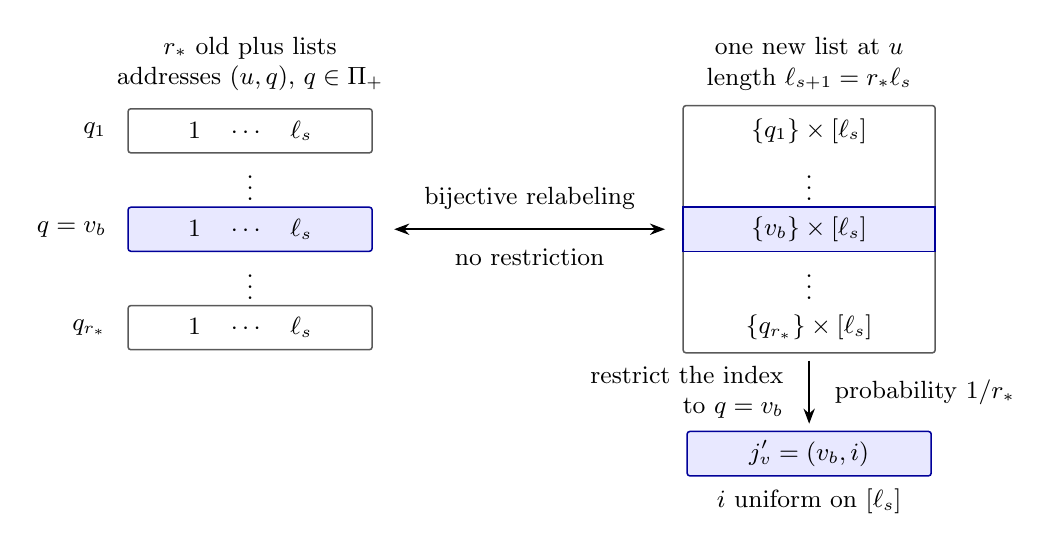
\begin{tikzpicture}[
  x=1cm,y=1cm,
  font=\small,
  list/.style={draw=black!65,rounded corners=1pt,
               minimum width=3.1cm,minimum height=.56cm},
  selected/.style={fill=blue!9,draw=blue!60!black},
  every path/.style={line width=.55pt}
]
  \node[align=center] at (1.55,.85)
    {$r_*$ old plus lists\\addresses $(u,q)$, $q\in\Pi_+$};
  \node[align=center] at (8.65,.85)
    {one new list at $u$\\length $\ell_{s+1}=r_*\ell_s$};

  \node[list] at (1.55,0) {$1\quad\cdots\quad\ell_s$};
  \node[anchor=east] at (-.15,0) {$q_1$};
  \node at (1.55,-.62) {$\vdots$};
  \node[list,selected] at (1.55,-1.25)
    {$1\quad\cdots\quad\ell_s$};
  \node[anchor=east] at (-.15,-1.25) {$q=v_b$};
  \node at (1.55,-1.88) {$\vdots$};
  \node[list] at (1.55,-2.5) {$1\quad\cdots\quad\ell_s$};
  \node[anchor=east] at (-.15,-2.5) {$q_{r_*}$};

  \draw[<->,>=Stealth] (3.38,-1.25)--(6.82,-1.25);
  \node[above,align=center] at (5.1,-1.13) {bijective relabeling};
  \node[below,align=center] at (5.1,-1.37) {no restriction};

  \draw[black!65,rounded corners=1pt] (7.05,.32) rectangle (10.25,-2.82);
  \node at (8.65,0) {$\{q_1\}\times[\ell_s]$};
  \node at (8.65,-.62) {$\vdots$};
  \filldraw[selected] (7.05,-.97) rectangle (10.25,-1.53);
  \node at (8.65,-1.25) {$\{v_b\}\times[\ell_s]$};
  \node at (8.65,-1.88) {$\vdots$};
  \node at (8.65,-2.5) {$\{q_{r_*}\}\times[\ell_s]$};

  \draw[->,>=Stealth] (8.65,-2.92)--(8.65,-3.72);
  \node[anchor=east,align=right] at (8.45,-3.32)
    {restrict the index\\to $q=v_b$};
  \node[anchor=west] at (8.85,-3.32) {probability $1/r_*$};
  \node[list,selected] at (8.65,-4.1) {$j'_v=(v_b,i)$};
  \node[below] at (8.65,-4.42) {$i$ uniform on $[\ell_s]$};
\end{tikzpicture}
\caption{Regrouping at a fixed new address
$u=u_{S\cup\{b\}}(v)$ and restricting the index of one slot $v\in V_+$.
The horizontal arrow only relabels the same independent entries; it
incurs no probability factor.  The highlighted sublist is prescribed
by $v_b$.  Restricting all $n_*$ independent slot indices to their
respective prescribed sublists has probability $r_*^{-n_*}$.
The ellipses denote the other words in $\Pi_+$; boxes describe index
positions, and their field values may coincide.}
\label{tuple:fig-regrouping}
\end{figure}


A new address edge requires $t+1$ shifted blocks outside $S'$.  Those blocks
also certify an old edge for every choice of the two words in block
$b$.  Hence every factor of $I_{S'}(Y')$ occurs, with its direction
unchanged, among the factors of $I_+(Y_+)$.  Since all factors belong
to $[0,1]$,
\[
 I_+(Y_+)\le I_{S'}(Y').
\]
When $S'$ is terminal this inequality follows from $I_{S'}=1$.

Apply \eqref{eq:4} to $S'$.  In its nonnegative right-hand side,
restrict the new index at each $v\in V_+$ to the sublist
$\{v_b\}\times[\ell_s]$.  Each restriction has probability $1/r_*$,
independently across the $n_*$ slots.  On this event the labels and
the remaining independent indices are exactly those in
$\mathcal D_S(J)$.  Its probability is $r_*^{-n_*}$, and the
pointwise weight comparison above now yields \eqref{eq:6}.
\end{proof}

\subsection{The mixture, its support, and covariance}

We can now choose the mixture.  The gain in \eqref{eq:6} is a fixed
positive constant, whereas the possible loss in \eqref{eq:5} tends
to zero with $p$.  Thus a component with one more marked block may
receive a smaller coefficient and still compensate for that loss.

\begin{proposition}[Reflection-positive laws with polynomial cycle support]
\label{tuple:laws}
For all sufficiently large primes $p$, uniformly in $l\ge1$, define
\begin{align*}
 M_{l,p}&=\sum_{\substack{S\subseteq[w]\\|S|\le t+1}}
                 p^{-|S|\delta/2}\nu_{l,p,S},\\
 \mu_{l,p}&=\frac{M_{l,p}}{M_{l,p}(1)},\\
 \eps_{l,p}&=\frac{1}{M_{l,p}(1)}
       \sum_{|S|=t+1}p^{-(t+1)\delta/2}\nu_{l,p,S}.
\end{align*}
Then $\mu_{l,p}$ is a reflection-positive probability law and
$0\le\eps_{l,p}\le\mu_{l,p}$.  Its exceptional mass satisfies
\[
 \eta_{l,p}:=\eps_{l,p}(1)\le p^{-4}.
\]
The probability law
\[
 \mu_{l,p}^{\circ}
       =\frac{\mu_{l,p}-\eps_{l,p}}{1-\eta_{l,p}}
\]
has only admissible increments $z_{v_{j+1}}-z_{v_j}$ along the
designated cycle.  Every component and both measures $\mu_{l,p}$,
$\eps_{l,p}$ are invariant under simultaneous translation of all
labels.  Every positive-mass component or subsum therefore has uniform
single-slot marginals after normalization.  In either $\mu_{l,p}$ or
$\mu_{l,p}^{\circ}$, the total probability of components with
$S\ne\varnothing$ is $O(p^{-\delta/2})$.
\end{proposition}

\begin{proof}
At a cut in block $b$, pair each $S$ with $b\notin S$, $|S|\le t$,
with $S\cup\{b\}$.  Each component containing $b$ appears in exactly
one pair.  Equations~\eqref{eq:5} and \eqref{eq:6} bound the quadratic
form of the pair below by
\[
 p^{-|S|\delta/2}
 \left(p^{-\delta/2}c_*r_*^{-n_*}-Cp^{-\delta}\right)
 \mathcal D_S(J).
\]
This is nonnegative once $p$ is sufficiently large.  The only unpaired
sets are terminal sets omitting $b$; their forms are nonnegative by
Lemma~\ref{tuple:unmarked-defect}.  Thus $M_{l,p}$ is reflection
positive at every cut.

For $S=\varnothing$, each list has length one and $R_S=1$.
Lemma~\ref{tuple:list-mixing} and $c_p\ge1/(2k)$ show that
$\nu_{\varnothing}(1)$ is bounded below by a fixed positive constant
for all sufficiently large $p$.  All component masses are bounded
above, and the number of components is fixed.  It follows that
\[
 0<c\le M_{l,p}(1)\le C,\qquad
 \eps_{l,p}(1)\le C p^{-(t+1)\delta/2}.
\]
Our choice $(t+1)\delta/2>5$ gives the stated bound $p^{-4}$ after
increasing the prime threshold.  Summing the nonleading coefficients
also gives total probability $O(p^{-\delta/2})$ for $S\ne\varnothing$.
Removing the terminal components retains the positive leading mass,
so the same estimate holds after normalization to $\mu_{l,p}^{\circ}$.

Simultaneous translation of all list entries preserves their product
law, all differences in $I_S$, and the index weight $R_S$.  It
therefore translates every output label and proves the asserted
invariances and marginal uniformity.

Finally, a nonterminal $S$ leaves at least $t+1$ blocks unmarked.
Consecutive cycle vertices shift by $c$ in all these blocks, including
the edge from $v_{L-1}$ to $v_0$.  Their addresses are consequently
joined by a directed edge.  Since its weights include every pair of
list entries, any positive-weight label tuple has admissible
increment on this edge, regardless of the chosen indices.  This
holds around the entire cycle in every component retained by
$\mu_{l,p}^{\circ}$.
\end{proof}

The auxiliary parameter changes the edge weight, so we need covariance
between different laws rather than dilation invariance of a single law.

\begin{lemma}[Covariance under progression changes]
\label{tuple:covariance}
For every $l\ge1$, every sufficiently large prime $p$, and every
integer $D\ge1$ with $p\nmid D$, the following holds.  For each
$a'\in\F_p$, the map
\begin{equation}
 (z_v)_{v\in V}\longmapsto
       \bigl(\lambda(D)^{-1}(z_v-a')\bigr)_{v\in V}
 \label{eq:7}
\end{equation}
pushes $\mu_{l,p}$ to $\mu_{lD,p}$ and $\eps_{l,p}$ to
$\eps_{lD,p}$.
\end{lemma}

\begin{proof}
Equation~\eqref{eq:1} states that
$h_l(Dx-i)=\lambda(D)h_{lD}(x)$.  Both $D$ and $\lambda(D)$ are
units modulo $p$.  The argument map $x\mapsto Dx-i$ is therefore a
bijection and, on differentiating this identity, preserves regularity.
Counting regular arguments gives
\[
 W_{lD,p}(y)=W_{l,p}(\lambda(D)y).
\]
Apply \eqref{eq:7} to every list entry in a component measure.  The
independent uniform list law and all index weights are unchanged;
each old edge weight becomes exactly the corresponding new edge
weight.  Thus the map pushes $\nu_{l,p,S}$ to $\nu_{lD,p,S}$ for
each $S$.  All component masses, and in particular the normalizing
masses $M_{l,p}(1)$ and $M_{lD,p}(1)$, agree.  The two claimed
pushforwards follow with no additional factor.
\end{proof}

\subsection{Conditional mixing and the prime threshold}

The mixture has the required positivity and support.  To control high
Fourier frequencies later, we also need to know that the other labels
give little information about a mean-zero function of any one label.
The leading component has this property by list mixing.  The remaining
components have small total probability, and their uniform marginals
give the bound needed to include them.

\begin{lemma}[Conditional mixing]
\label{tuple:conditional-mixing}
For all sufficiently large $p$, uniformly in $l$, let $\rho_p$ be
either $\mu_{l,p}$ or $\mu_{l,p}^{\circ}$.  For every $v\in V$ and
every function $f:\F_p\to\C$ of uniform mean zero,
\begin{equation}
 \left\|\E_{\rho_p}\bigl(f(z_v)\mid
                         (z_{v'})_{v'\ne v}\bigr)\right\|_2
       \le p^{-\gamma}\|f\|_2.
 \label{eq:8}
\end{equation}
The norm on the left is taken in the other-label marginal of
$\rho_p$; the norm on the right is uniform on $\F_p$.
\end{lemma}

\begin{proof}
First normalize the leading component $\nu_{\varnothing}$, and
write $x=z_v$, $y=(z_{v'})_{v'\ne v}$.  Before normalization its
density relative to uniform labels is $K_1(x,y)K_2(y)$, where $K_1$
is the product of the $m$ weights on edges incident to $v$, and
$K_2$ contains the remaining weights.  Put
\[
 A(y)=\E_xK_1(x,y),\qquad
 B_f(y)=\E_x f(x)K_1(x,y).
\]
The incident edges form a graph between the singleton list $x$ and
the list $y$.  Equation~\eqref{eq:3}, applied to this kernel, gives
\[
 \|A-c_p^m\|_2\ll p^{-\delta},\qquad
 \|B_f\|_2\ll p^{-\delta}\|f\|_2.
\]
This includes $m=0$, when $A=1$ and $B_f=0$.

Let $Z_0=\nu_{\varnothing}(1)$, which is bounded below uniformly.
The other-label marginal has density $Z_0^{-1}K_2(y)A(y)$, and the
conditional expectation equals $B_f(y)/A(y)$ where $A(y)>0$.
Its squared norm is therefore exactly
\[
 \frac1{Z_0}\E_y K_2(y)\frac{|B_f(y)|^2}{A(y)},
\]
with the ratio taken as zero if $A(y)=0$.  On $A\ge c_p^m/2$, the
bound on $B_f$ makes this $O(p^{-2\delta})\|f\|_2^2$.  The
complement has uniform probability $O(p^{-2\delta})$, by the bound
on $A-c_p^m$ and the fixed positive lower bound on $c_p^m$.
Everywhere, weighted Cauchy--Schwarz gives
\[
 \frac{|B_f(y)|^2}{A(y)}
       \le\E_x |f(x)|^2K_1(x,y)\le\|f\|_2^2.
\]
Since $K_2\le1$, the complement has the same required bound.  Thus
the squared conditional norm in the normalized leading component is
$O(p^{-2\delta})\|f\|_2^2$.

For either mixture, condition additionally on its component index.
The tower property and Jensen's inequality can only increase the
squared conditional norm under this extra conditioning.  In each
nonleading component the trivial bound is $\|f\|_2^2$, because its
single-slot marginal is uniform.  Proposition~\ref{tuple:laws} bounds
their total probability by $O(p^{-\delta/2})$.  The squared norm for
the mixture is consequently $O(p^{-\delta/2})\|f\|_2^2$, and the
norm is $O(p^{-\delta/4})\|f\|_2$.  Since $\gamma=\delta/10$, the
fixed implicit constant is absorbed by taking $p$ sufficiently large,
proving \eqref{eq:8}.
\end{proof}

We require a threshold $P>P_1$ such that all the preceding
assertions hold for every prime $p\ge P$, uniformly in $l$.  We
further require
\begin{equation}
 3\le p^{\gamma/2}\quad(p\ge P),\qquad
 \prod_{\substack{p\ge P\\p\ \mathrm{prime}}}(1+p^{-3})-1
       \le\frac14.
 \label{eq:9}
\end{equation}
The second requirement is possible by convergence of the product.
For such a choice, define the small-prime modulus
\[
 M_0=\prod_{\substack{p<P\\p\ \mathrm{prime}}}p^{E_p}\ge2,
\]
using the exponents $E_p$ from Section~\ref{sec:local}.  If a modulus
is $M_0$ times a squarefree product of primes at least $P$, a residue
modulo that modulus is called admissible for $l$ when it is admissible
at each of its local prime-power factors.  This convention combines
the small-prime lifting conditions with the cycle support supplied
by Proposition~\ref{tuple:laws}.

\subsection{Dependence of the tuple threshold}

To obtain an exponent depending only on the degree, we need the tuple
threshold to be uniform when the local choices are uniform.  The next
proposition traces that dependence while retaining the construction for
general fixed polynomial data.

\begin{proposition}[Dependence of the prime threshold]
\label{tuple:threshold-dependence}
For the auxiliary family and local choices above, the threshold $P$ can
be chosen as a function of $k,P_1,L,t$ alone so that
Proposition~\ref{tuple:laws}, Lemmas~\ref{tuple:covariance}
and~\ref{tuple:conditional-mixing}, and \eqref{eq:9} hold uniformly in
$l$.  For general fixed data, $P_1$ may depend on $h$, and $L$ may depend
on $h$ and its chosen roots.  If $h$ satisfies Condition~\eqref{local:unit-condition}
and the degree-dependent choices of $P_1$, $E_p$, and $L$ from
Section~\ref{sec:local} are used, then $P$ and $M_0$ depend only on $k$.
\end{proposition}

\begin{proof}
For every prime $p\ge P_1$, the quantitative local input to the estimates
above is
\[
 0\le W_{l,p}\le1,\qquad c_p\ge(2k)^{-1},\qquad
 \max_{u\ne0}|\widehat W_{l,p}(u)|\le p^{-4\delta}.
\]
Indeed, with the normalized Fourier convention, for $u\ne0$ the coefficient
$\widehat W_{l,p}(u)$ is $c_p$ times the corresponding regular-argument
average in \eqref{eq:2}; also $c_p\le1$.  These statements hold uniformly
in $l$.  We extract
constants from the preceding proofs using
\[
 e_*:=\binom d2,\qquad R_*:=\exp(e_*),\qquad
 C_{\mathrm{gr}}:=(32e_*)^{1/4},\qquad
 Z_*:=\frac12(2k)^{-e_*}.
\]
They depend only on $k,L,t$, since $d=(L!)^{2t+1}$.

For a set of $s$ marked blocks, the graph on list entries has
$K^{w-s}\ell_s=d/2^s\le d$ formal vertices.  Its simplicity was checked
above before field labels were assigned, so coincidences between their
values do not affect the graph bound.  Every graph for $I_S$, every
cross-list graph in Lemma~\ref{tuple:unmarked-defect}, and every incident
graph in Lemma~\ref{tuple:conditional-mixing} consequently has at most
$e_*$ edges.  Lemma~\ref{tuple:list-mixing} therefore bounds their graph
errors by $e_*p^{-4\delta}$.  For the cross-list and incident graphs,
which join two lists, it bounds the operator errors by
$C_{\mathrm{gr}}p^{-\delta}$.

Each index interaction $H^S_{xy}$ is at most one, so $R_S$ and every
within-half weight $R_+$ are at most $R_*$.  In particular,
$\nu_S(1)\le R_*$.  The proof of Lemma~\ref{tuple:marked-positive} gives
the explicit constant
\[
 c_*=(\exp(\kappa)-1)^{n_*}\ell_{t+1}^{-n_*},
 \qquad
 \kappa=\frac9{10}(10L^2)^{-(L-1)}.
\]
The exact half-index factor $\ell_s^{-n_*}$ proved there and the exact
index-restriction factor $r_*^{-n_*}$ in
Lemma~\ref{tuple:marking-domination} give the domination constant
$c_*r_*^{-n_*}$.  In the unmarked
proof, Cauchy--Schwarz and $I_+^2\le I_+$ give
$\|g\|_2^2\le R_*^2\mathcal D_S(J)$.  The list bound just obtained thus
allows the constant in \eqref{eq:5} to be
\[
 C_{\mathrm{def}}:=R_*^2C_{\mathrm{gr}}.
\]
The pairing proof of Proposition~\ref{tuple:laws} is therefore
nonnegative at every cut whenever
\[
 p^{\delta/2}\ge C_{\mathrm{def}}r_*^{n_*}/c_*.
\]

Let $e_0\le e_*$ be the number of edges in the leading component.
The graph estimate and the lower bound on $c_p$ give
\[
 \nu_{\varnothing}(1)
 \ge c_p^{e_0}-e_0p^{-4\delta}
 \ge (2k)^{-e_*}-e_*p^{-4\delta}.
\]
Consequently $\nu_{\varnothing}(1)\ge Z_*$ once
$e_*p^{-4\delta}\le Z_*$.  There are at most $2^w$ components, each of
mass at most $R_*$.  Set
\[
 C_{\mathrm{mass}}:=\frac{2^wR_*}{Z_*},\qquad
 \alpha_{\mathrm{exc}}:=\frac{(t+1)\delta}{2}>5.
\]
The normalizing mass $M_{l,p}(1)$ is at least the leading mass, so
\[
 \eta_{l,p}\le C_{\mathrm{mass}}p^{-\alpha_{\mathrm{exc}}}.
\]
It is at most $p^{-4}$ if
$p^{\alpha_{\mathrm{exc}}-4}\ge C_{\mathrm{mass}}$.  In either
$\mu_{l,p}$ or $\mu_{l,p}^{\circ}$ the probability of nonleading
components is at most $C_{\mathrm{mass}}p^{-\delta/2}$.  For the latter
law, its unnormalized mass after removing the terminal terms still
contains $\nu_{\varnothing}(1)\ge Z_*$; hence the same denominator
bound applies without an additional normalization factor.  Cycle support
and translation invariance in Proposition~\ref{tuple:laws} are exact
properties of these components and impose no further threshold.

For the leading component in Lemma~\ref{tuple:conditional-mixing}, the
incident graph has $m\le e_*$ edges.  Its list operator error is at most
$C_{\mathrm{gr}}p^{-\delta}$.  The split into $A\ge c_p^m/2$ and its
complement in that proof therefore bounds the squared conditional norm by
\[
 Z_0^{-1}C_{\mathrm{gr}}^2
 \bigl(2c_p^{-m}+4c_p^{-2m}\bigr)p^{-2\delta}\|f\|_2^2.
\]
Using $Z_0\ge Z_*$ and $c_p^{-m}\le(2k)^{e_*}$ bounds this by
\[
 C_{\mathrm{lead}}p^{-2\delta}\|f\|_2^2,
 \qquad
 C_{\mathrm{lead}}:=Z_*^{-1}C_{\mathrm{gr}}^2
 \bigl(2(2k)^{e_*}+4(2k)^{2e_*}\bigr).
\]
The case $m=0$ already has zero conditional norm.  For either mixture,
conditioning additionally on the component index and applying Jensen's
inequality bounds its squared conditional norm by
\[
 \bigl(C_{\mathrm{lead}}p^{-2\delta}
       +C_{\mathrm{mass}}p^{-\delta/2}\bigr)\|f\|_2^2
 \le (C_{\mathrm{lead}}+C_{\mathrm{mass}})
       p^{-\delta/2}\|f\|_2^2.
\]
Here the bound in every other component is $\|f\|_2^2$ because its
single-slot marginal is uniform.  As
$\delta/2-2\gamma=3\delta/10>0$, the desired squared bound
$p^{-2\gamma}\|f\|_2^2$ follows once
\[
 p^{\delta/2-2\gamma}\ge C_{\mathrm{lead}}+C_{\mathrm{mass}}.
\]

Choose an integer $P>P_1$ large enough that the displayed requirements
on $p$ above hold for every $p\ge P$, and that $P^{\gamma/2}\ge3$.
This is possible because $\delta>0$, $\alpha_{\mathrm{exc}}-4>0$, and
$\delta/2-2\gamma>0$, and all the constants depend only on $k,L,t$.
The product condition in \eqref{eq:9} can be
included in the same choice: for integer $P\ge2$,
\[
 \prod_{\substack{p\ge P\\p\ \mathrm{prime}}}(1+p^{-3})
 \le \exp\left(\sum_{n\ge P}n^{-3}\right)
 \le \exp\left(\frac{1}{2(P-1)^2}\right),
\]
whose last expression tends to one.  The covariance proof uses only the
exact progression identity and bijections when $p\nmid D$, so it imposes
no further restriction on $P$.  This proves the stated dependence of $P$.
Under Condition~\eqref{local:unit-condition}, Section~\ref{sec:local}
allows $P_1,L$ to be chosen from $k$ and each $E_p$ from $k,p$.  Also,
$t$ is chosen from $\delta$, which depends only on $k$.  The product defining $M_0$
then uses a degree-dependent set of primes and degree-dependent
exponents.  For a general fixed polynomial, $M_0$ retains any dependence
of the local exponents $E_p$ as well as that of $P_1$ and $L$.
\end{proof}

For the rest of the paper, fix a choice of $P$ supplied by
Proposition~\ref{tuple:threshold-dependence} and the corresponding $M_0$.

\section{Multilinear estimates and Fourier lifts}
\label{sec:lifts}

The tuple laws of Section~\ref{sec:tuples} provide two ways to control
multilinear averages: reflection positivity compares different inputs
with a single diagonal quantity, while conditional mixing suppresses
large Fourier denominators.  We develop both estimates, then prove the
moment bounds needed to apply them to bounded functions on integer
intervals.  The signed-form estimates adapt~\cite[Proposition~4.1 and
Lemmas~4.2--4.3]{squarepower}.  We prove the needed estimates for the
present laws, with changes of auxiliary parameter replacing the dilation
invariance used in the square setting.

Retain the index set \(V=\Pi^w\), where \(\Pi\) consists of the
permutation words on \([L]\), and put \(d=|V|\); in particular, \(d\) is even.
Fix a positive integer
\(l\) and a finite set \(\mathcal P\) of primes at least \(P\).  Set
\[
 X_{\mathcal P}=\prod_{p\in\mathcal P}\F_p,
 \qquad
 \mu_{l,\mathcal P}=\bigotimes_{p\in\mathcal P}\mu_{l,p}.
\]
We collect the prime labels in slot \(v\) into a single variable
\(z_v\in X_{\mathcal P}\), so \(\mu_{l,\mathcal P}\) is a probability
law on \(X_{\mathcal P}^V\).  Each single-slot marginal is uniform.
Norms of functions on \(X_{\mathcal P}\) will always use uniform
probability measure unless another measure is specified.
For real functions on this space define
\[
 \mathcal Z_{l,\mathcal P}((g_v)_{v\in V})
 =\int\prod_{v\in V}g_v(z_v)\,d\mu_{l,\mathcal P},
 \qquad
 Z_{l,\mathcal P}(g)=\mathcal Z_{l,\mathcal P}((g)_{v\in V}).
\]
The empty prime set is allowed: its residue space is a singleton and
\(Z_{l,\varnothing}(g)=g^d\).

We also fix the Fourier notation on these spaces.  Every frequency has a
unique additive decomposition
\[
 \xi=\sum_{p\in\mathcal P}\frac{a_p}{p}\pmod 1,
 \qquad 0\le a_p<p,
\]
and its character is
\(e(z\xi)=\prod_{p\in\mathcal P}e(a_pz_p/p)\).
Equivalently, one may use any integer representative of \(z\) supplied
by the Chinese remainder theorem.  The \emph{exact support} of this
character is \(\{p:a_p\ne0\}\); its reduced denominator is the product
of those primes.  For \(B\subseteq\mathcal P\) write
\(q_B=\prod_{p\in B}p\), with \(q_\varnothing=1\).

\subsection{Signed H\"older inequality and seminorm rules}

The finite reflection argument below follows the chessboard method of
Fr\"ohlich, Israel, Lieb and Simon~\cite[Theorem~4.1]{FILS1978};
related reflection arguments for graph norms appear in Conlon and
Lee~\cite[Section~3]{ConlonLee2017}.
The standard passage from a multilinear H\"older inequality to a seminorm
is also part of Hatami's criterion for graph norms~\cite[Theorem~2.8 of
the arXiv version]{Hatami2010}; we prove both steps directly for the
present tuple laws.

\begin{proposition}[Signed H\"older inequality]
\label{lift:signed-holder}
For every positive integer \(l\), finite set \(\mathcal P\) of primes
at least \(P\), and real functions \(g,g_v:X_{\mathcal P}\to\R\),
\begin{equation}
 Z_{l,\mathcal P}(g)\ge0,
 \qquad
 \left|\mathcal Z_{l,\mathcal P}((g_v)_{v\in V})\right|
 \le\prod_{v\in V} Z_{l,\mathcal P}(g_v)^{1/d}.
 \label{eq:10}
\end{equation}
\end{proposition}

\begin{proof}
Across any reflection cut of \(V\), the matrix of the product law is
the tensor product of the corresponding prime-law matrices.  It is
therefore positive semidefinite.  To explain its consequence for signed
inputs, fix a cut \(V=V_+\sqcup V_-\) and its reflection \(\theta\).
Define maps \(\phi_\pm:V\to V_\pm\) that fix the selected half and
reflect the other half into it.  An assignment of functions is a map
\(a:v\mapsto g_v\); write its integral as \(\Lambda(a)\).
The two real functions on the plus-half labels that enter the cut
bilinear form are
\[
 F(x)=\prod_{v\in V_+}a(v)(x_v),
 \qquad
 G(x)=\prod_{v\in V_+}a(\theta v)(x_v).
\]
Its mixed value is \(\Lambda(a)\), and its two quadratic values are
\(\Lambda(a\circ\phi_+)\) and \(\Lambda(a\circ\phi_-)\).
Cauchy--Schwarz for the positive semidefinite matrix gives
\begin{equation}
 |\Lambda(a)|^2
 \le \Lambda(a\circ\phi_+)\Lambda(a\circ\phi_-),
 \qquad \Lambda(a\circ\phi_\pm)\ge0.
 \label{lift:fold-cs}
\end{equation}
In particular a constant assignment has nonnegative integral, proving
the first assertion of~\eqref{eq:10}.

We next give a finite sequence of fold maps that sends every vertex to
one vertex.  In one block write \(p_i\) for the position of symbol
\(i\) in its permutation word.  Folding onto the half where \(i\)
precedes \(i+1\) sorts the pair \((p_i,p_{i+1})\), leaving all other
entries unchanged.  Apply the comparisons \(i=1,\ldots,L-1\) in that
order, and repeat this sweep \(L-1\) times.  A sweep moves the largest
entry to the end.  Once the largest entries occupy their final positions,
the next sweep leaves them there and places the largest remaining entry
immediately before them.  Thus every position array becomes
\((1,\ldots,L)\).  Perform these sweeps in each block.  If their fold
maps in chronological order are \(\phi_1,\ldots,\phi_m\), then
\[
 \phi_m\circ\cdots\circ\phi_1(v)=v_*
 \quad\text{for every }v\in V,
\]
where \(v_*\) has the identity word in every block.

Now fix a finite nonempty list of real functions and let \(M\) be the
maximum absolute integral over all assignments from that list, allowing
repetition.  If \(M>0\), take a maximizing assignment.  Each of its
folded integrals is nonnegative and at most \(M\), while their product
is at least \(M^2\) by~\eqref{lift:fold-cs}.  Both therefore equal
\(M\).  Hence either fold preserves maximality.  Apply the pullbacks
in reverse order, first \(\phi_m\), then \(\phi_{m-1}\), and so on.
The final assignment is
\(a\circ\phi_m\circ\cdots\circ\phi_1\), which is constant.  It
follows that \(M\) is a diagonal value.  Conversely, constant
assignments are included in the maximum.  We have proved that the
maximum absolute mixed integral equals the largest diagonal value in
the list; this is also true when \(M=0\).

For \(\epsilon>0\), apply this conclusion to the list
\[
 \frac{g_v}{(Z_{l,\mathcal P}(g_v)+\epsilon)^{1/d}},
 \qquad v\in V.
\]
Each diagonal value in this list is at most one.  Multilinearity gives
\( |\mathcal Z_{l,\mathcal P}((g_v)_v)|
 \le\prod_v(Z_{l,\mathcal P}(g_v)+\epsilon)^{1/d}\).
Let \(\epsilon\downarrow0\).  This proves the second assertion,
including cases where some diagonal values vanish.
\end{proof}

Define
\[
 \|g\|_{l,\mathcal P}=Z_{l,\mathcal P}(g)^{1/d}
 \quad\text{for real }g.
\]
For \(B\subseteq\mathcal P\), let \(\E_B g\) mean uniform averaging
over the coordinates in \(B\), with all other coordinates held fixed.
The resulting function may be viewed on either \(X_{\mathcal P}\) or
\(X_{\mathcal P\setminus B}\).

\begin{lemma}[Seminorm and changes of coordinates]
\label{lift:seminorm}
The map \(g\mapsto\|g\|_{l,\mathcal P}\) is a seminorm on the real
functions on \(X_{\mathcal P}\).  It satisfies
\[
 |\E g|\le\|g\|_{l,\mathcal P},
 \qquad
 \|\E_Bg\|_{l,\mathcal P\setminus B}
 =\|\E_Bg\|_{l,\mathcal P}
 \le\|g\|_{l,\mathcal P}.
\]
Translations of the input are isometries.  Moreover, if \(D\) is a
positive integer coprime to every prime of \(\mathcal P\), then for
any \(a'\in X_{\mathcal P}\),
\begin{equation}
 \left\|g\bigl(\lambda(D)^{-1}(\,\cdot-a')\bigr)
       \right\|_{l,\mathcal P}
 =\|g\|_{lD,\mathcal P}.
 \label{lift:transport}
\end{equation}
Here the affine change is interpreted separately at each prime.
\end{lemma}

\begin{proof}
Nonnegativity follows from Proposition~\ref{lift:signed-holder}.
Since \(d\) is even, homogeneity of \(Z\) gives absolute homogeneity
of its \(d\)-th root.  Expanding \(Z(g+h)\) by its slots and applying
\eqref{eq:10} termwise gives
\[
 Z_{l,\mathcal P}(g+h)
 \le\sum_{S\subseteq V}\|g\|_{l,\mathcal P}^{|S|}
                         \|h\|_{l,\mathcal P}^{d-|S|}
 =\bigl(\|g\|_{l,\mathcal P}+\|h\|_{l,\mathcal P}\bigr)^d.
\]
Taking roots proves the triangle inequality.
Putting \(g\) in one slot and 1 in all others in~\eqref{eq:10}
proves mean domination, since the single-slot marginal is uniform and
\(Z(1)=1\).

The simultaneous translation invariance of the tuple laws proves that
translations are isometries.  Let \(G_B\subseteq X_{\mathcal P}\)
be the additive subgroup of vectors supported on \(B\).  Then
\[
 (\E_Bg)(z)=\frac1{|G_B|}\sum_{a\in G_B}g(z+a).
\]
The triangle inequality gives the asserted contraction.  Since
\(\E_Bg\) is independent of \(B\), the probability laws at those
primes integrate out, proving the equality of the two seminorms.
Finally, \(\lambda(D)\) is a unit at each remaining prime, and
\eqref{eq:7} pushes the product law at \(l\) exactly to that at
\(lD\).  This proves~\eqref{lift:transport}.
\end{proof}

\subsection{Decay at large Fourier denominators}

Conditional mixing gives a different estimate, valid also after
removing the exceptional part of each prime law.  Its proof requires
orthogonality between different exact supports; applying the triangle
inequality to all Fourier coefficients would lose this decay.

\begin{lemma}[Large-denominator estimate]
\label{lift:large-denominator}
Fix \(l\ge1\) and a finite prime set \(\mathcal P\) as above.  At
each prime choose either \(\rho_p=\mu_{l,p}\) or
\(\rho_p=\mu_{l,p}^{\circ}\).  Let \(g_v:X_{\mathcal P}\to\C\)
be arbitrary functions.  If, in one distinguished slot \(v\), every
Fourier coefficient at a denominator at most \(R\) vanishes, where
\(R\ge1\), then
\begin{equation}
 \left|\int\prod_{u\in V}g_u(z_u)\,
                  d\bigotimes_{p\in\mathcal P}\rho_p\right|
 \le R^{-\gamma}\|g_v\|_2
                     \prod_{u\ne v}\|g_u\|_{2(d-1)}.
 \label{eq:11}
\end{equation}
\end{lemma}

\begin{proof}
At one prime, let \(\mathfrak m_p\) denote the marginal law of the labels in all
slots other than \(v\), and let
\[
 T_p f=\E_{\rho_p}\bigl(f(z_v)\mid(z_u)_{u\ne v}\bigr).
\]
This is an operator from uniform \(L^2(\F_p)\) to \(L^2(\mathfrak m_p)\).
It preserves constants.  It sends uniform-mean-zero inputs to
\(\mathfrak m_p\)-mean-zero outputs, since \(\E_{\mathfrak m_p}T_pf=\E f\).
By~\eqref{eq:8}, its norm on the mean-zero subspace is at most
\(p^{-\gamma}\).

The product law makes the conditional operator for all primes equal
to \(T=\bigotimes_pT_p\): this identity holds first for products of
one-prime functions, by independence across primes, and then for every
function by linearity.  The exact-support \(B\) Fourier space has a
mean-zero factor at primes in \(B\) and a constant factor elsewhere.
On this space the operator norm is at most \(q_B^{-\gamma}\).
Furthermore, the images of two distinct exact-support spaces are
orthogonal in \(L^2(\bigotimes_p\mathfrak m_p)\).  At a prime in the symmetric
difference of the supports, one image factor is constant and the other
has mean zero.  Their inner product is zero, and tensoring preserves
this orthogonality.

Decompose \(g_v=\sum_{q_B>R}g_{v,B}\) by exact supports.  Both the
domain summands and their images are orthogonal, so
\[
 \|Tg_v\|_2^2
 =\sum_{q_B>R}\|Tg_{v,B}\|_2^2
 \le\sum_{q_B>R}q_B^{-2\gamma}\|g_{v,B}\|_2^2
 \le R^{-2\gamma}\|g_v\|_2^2.
\]
Condition the original integral on the other slots and apply
Cauchy--Schwarz.  The remaining factor is bounded by
\[
 \left\|\prod_{u\ne v}g_u(z_u)\right\|_2
 \le\prod_{u\ne v}
       \left(\E|g_u(z_u)|^{2(d-1)}\right)^{1/(2(d-1))}
 =\prod_{u\ne v}\|g_u\|_{2(d-1)},
\]
using ordinary H\"older and the uniform single-slot marginals.
This proves~\eqref{eq:11}.  If \(\mathcal P\) is empty, the frequency
hypothesis forces \(g_v=0\), and the conclusion is immediate.
\end{proof}

\subsection{Fourier lifts and uniform moments}

A bounded function on an integer interval gives Fourier coefficients at
rational frequencies.  We transfer a finite set of these coefficients
to \(X_{\mathcal P}\).  Such a transfer need not preserve pointwise
bounds, so we prove bounds for every fixed moment, following the
Fourier-lift argument of~\cite[Lemmas~5.1--5.2]{squarepower}.  We must also allow
arbitrary subfamilies of complete exact supports, because fixing some
residue coordinates changes which denominators remain.

Let \(I\) be a nonempty consecutive interval of integers and let
\(f:I\to\C\).  Put
\[
 \widehat f_I(\xi)=\frac1{|I|}\sum_{x\in I}f(x)e(-x\xi).
\]
For \(B\subseteq\mathcal P\), define its exact-support contribution
\[
 f_B(z)=\sum_{q(\xi)=q_B}\widehat f_I(\xi)e(z\xi),
\]
where the frequencies are characters of \(X_{\mathcal P}\).  For
\(Q\ge1\), the Fourier lift is
\[
 \mathcal L_{I,\mathcal P,Q}f(z)
 =\sum_{\substack{B\subseteq\mathcal P\\q_B\le Q}}f_B(z)
 =\sum_{\substack{\xi\text{ on }X_{\mathcal P}\\q(\xi)\le Q}}
                   \widehat f_I(\xi)e(z\xi).
\]
Each \(f_B\) depends only on the coordinates in \(B\), and has mean
zero in each of those coordinates.  If \(f\) is real, all these
functions are real because each summation set is closed under negation.
Retaining a support \(B\) always means retaining all its frequencies.

\begin{proposition}[Uniform lift moments]
\label{lift:moments}
Let \(\mathcal P\) be any finite set of primes, \(Q\ge1\), and let
\(I\) be a consecutive integer interval with \(|I|\ge10Q^6\).
For every integer \(r\ge1\), every \(\epsilon>0\), every function
\(f:I\to\C\), and every subfamily
\(\mathcal F\subseteq\{B\subseteq\mathcal P:q_B\le Q\}\),
\begin{equation}
 \left\|\sum_{B\in\mathcal F}f_B\right\|_{2r}
 \le C_{r,\epsilon}\|f\|_\infty Q^\epsilon.
 \label{eq:12}
\end{equation}
The constant is independent of the prime set, the interval and its
location, the function, and the subfamily.
\end{proposition}

\begin{proof}
The zero function is immediate; otherwise scale so that
\(\|f\|_\infty\le1\).  Write \(N_I=|I|\), and let \(u\) be the
largest cardinality of a support whose prime product is at most \(Q\).
We first control conditional sums of squares of the \(f_B\), then their
square-function moments.  Symmetrization will recover the moment of
their sum.

\smallskip
\noindent\emph{Conditional energy.}
For \(J\subseteq\mathcal P\) with \(q_J\le Q\), and any fixed
coordinate vector \(z_J\), we claim that
\begin{equation}
 \sum_{\substack{B\in\mathcal F\\B\supseteq J}}
       \E\bigl(|f_B|^2\mid z_J\bigr)\ll4^{|J|}.
 \label{eq:13}
\end{equation}
The conditional expectation here averages uniformly over all coordinates
outside \(J\).  If \(B\supseteq J\), the coefficient of an outside
character \(\eta\) of exact support \(B\setminus J\), after fixing
\(z_J\), is
\[
 c_J(\eta;z_J)
 =\frac1{N_I}\sum_{x\in I}f(x)e(-x\eta)
       \prod_{p\in J}\bigl(p\1_{\{x\equiv z_p\pmod p\}}-1\bigr).
\]
Indeed, the sum over the nonzero frequencies at \(p\) is
\(\sum_{a=1}^{p-1}e(a(z_p-x)/p)
=p\1_{\{x\equiv z_p\pmod p\}}-1\).
Different supports \(B\supseteq J\) have disjoint sets of outside
characters.  Conditional Parseval therefore identifies the left side of
\eqref{eq:13} with the squared Euclidean norm of this coefficient vector
on the union of those character sets.

Expand the product in \(c_J\) over subsets \(J'\subseteq J\).
Apart from a sign, the corresponding vector has coordinates
\[
 \frac{q_{J'}}{N_I}
 \sum_{\substack{x\in I\\x\equiv z_{J'}\pmod{q_{J'}}}}
                   f(x)e(-x\eta).
\]
The congruence denotes the class determined by the fixed coordinates in
\(J'\); for the empty subset it imposes no restriction.  Write its
progression as \(x=a+q_{J'}n\), with \(n\) in a consecutive interval
of length \(N'\).  Then
\[
 N'\ge0.9N_I/q_{J'},
 \qquad N'q_{J'}/N_I\le1.1.
\]
In these coordinates the frequencies are \(q_{J'}\eta\), up to
constant phases.  They remain distinct because their denominators are
coprime to \(q_J\).  Their denominators are at most \(Q\), so they
number at most \(Q^2\) and have pairwise circle distance at least
\(Q^{-2}\).

The Gram matrix of these characters in normalized \(L^2\) on the
progression has diagonal 1.  By geometric summation, every off-diagonal
entry has modulus at most \(Q^2/(2N')\).  Its operator norm is
therefore at most its maximum absolute row sum, which is bounded by
\[
 1+\frac{Q^4}{2N'}
 \le1+\frac{Q^5}{1.8N_I}
 \le1+\frac1{18Q}.
\]
The associated Fourier analysis map has norm squared equal to this
Gram-matrix norm.  Since \(\|f\|_\infty\le1\) and
\(N'q_{J'}/N_I\le1.1\), the displayed coefficient vector has
Euclidean norm bounded by an absolute constant.  The triangle inequality
over the \(2^{|J|}\) subsets \(J'\), followed by squaring, proves
\eqref{eq:13}.

\smallskip
\noindent\emph{Square-function moments.}
Set
\[
 S(z)=\left(\sum_{B\in\mathcal F}|f_B(z)|^2\right)^{1/2}.
\]
Expand \(\E S^{2r}\) and fix the supports of its first \(r-1\)
factors.  Their union \(W'\) has size at most \((r-1)u\), and their
product depends only on \(z_{W'}\).  For the final support \(B\),
integration outside \(W'\) leaves exactly
\(\E(|f_B|^2\mid z_J)\), where \(J=B\cap W'\).
Every intersection that occurs satisfies \(q_J\le q_B\le Q\).
For each fixed intersection \(J\), the sum over supports with
\(B\cap W'=J\) is bounded by the larger sum over all \(B\supseteq J\)
in~\eqref{eq:13}.  There are at most \(2^{(r-1)u}\) possible
intersections and each has at most \(u\) elements.  Thus
\[
 \E S^{2r}\le C\,2^{(r-1)u}4^u\E S^{2r-2}.
\]
The same argument with \(r=1\) uses \(J=W'=\varnothing\).
Iteration gives
\begin{equation}
 \|S\|_{2r}\le C_r^{1+u}.
 \label{lift:square-function}
\end{equation}
The overlaps among supports have now been controlled.  It remains to
bound their sum by this square function with a loss exponential only in
\(u\).

\smallskip
\noindent\emph{Recovering the sum.}
Fix a support size \(j\ge1\) and color every prime coordinate with one
of \(j\) colors.  Call a support \emph{transversal} when it has exactly
one prime of each color, and let \(\mathcal T\) be the transversal
supports in \(\mathcal F\) for this coloring.  Take independent uniform
pairs \(X_p^0,X_p^1\) at every prime.  The operator
\(\operatorname{swap}_p\) interchanges these two copies.  Define
\[
 D_B=\prod_{p\in B}(1-\operatorname{swap}_p)f_B(X^0),
 \qquad B\in\mathcal T.
\]
Averaging over all second copies leaves \(f_B(X^0)\), since every
other term in this expansion has mean zero in at least one copied
coordinate.  Jensen's inequality gives
\[
 \left\|\sum_{B\in\mathcal T}f_B\right\|_{2r}
 \le\left\|\sum_{B\in\mathcal T}D_B\right\|_{L^{2r}(X^0,X^1)}.
\]
Independent swaps preserve the joint law of the copies and multiply
\(D_B\) by the product of the corresponding signs.  Thus for independent
uniform signs \(\epsilon_p\), indexed by primes,
\[
 \left\|\sum_{B\in\mathcal T}D_B\right\|_{L^{2r}(X^0,X^1)}
 =\left\|\sum_{B\in\mathcal T}D_B\prod_{p\in B}\epsilon_p
       \right\|_{L^{2r}(X^0,X^1,\epsilon)}.
\]

For completeness, the scalar sign estimate
\[
 \left\|\sum_i a_i\epsilon_i\right\|_{2r}
 \le C_r\left(\sum_i|a_i|^2\right)^{1/2}
\]
follows by expanding the even moment.  Surviving terms have even
multiplicity at every index.  For nonnegative coefficients their sum is
at most
\[
 \frac{(2r)!}{2^r r!}\left(\sum_i a_i^2\right)^r,
\]
because \((2m)!\ge2^m m!\).  For complex coefficients, take absolute
values of the surviving terms in
\((\sum_i a_i\epsilon_i)^r(\sum_i\overline{a_i}\epsilon_i)^r\)
and use the nonnegative case.  Iterating this estimate over the color
classes gives, for fixed copies,
\[
 \left\|\sum_{B\in\mathcal T}D_B\prod_{p\in B}\epsilon_p
       \right\|_{L^{2r}(\epsilon)}
 \le C_r^j\left(\sum_{B\in\mathcal T}|D_B|^2\right)^{1/2}.
\]
At each step Minkowski is used in the form
\(\| (\sum_i|B_i|^2)^{1/2}\|_{2r}
\le(\sum_i\|B_i\|_{2r}^2)^{1/2}\).
The signs are indexed by individual primes; transversality ensures that
each monomial uses exactly one sign from each color class.

In expanding the swaps in \(D_B\), index its \(2^j\) terms by a choice
of copy for each color.  For any fixed such choice, made consistently
across all supports, the selected prime coordinates have the original
product law.  The triangle inequality in
\(L^{2r}(\ell^2(\mathcal T))\) therefore gives
\[
 \left\|\left(\sum_{B\in\mathcal T}|D_B|^2\right)^{1/2}\right\|_{2r}
 \le2^j\left\|\left(\sum_{B\in\mathcal T}|f_B|^2\right)^{1/2}
       \right\|_{2r}
 \le2^j\|S\|_{2r}.
\]
Consequently the transversal sum has norm at most
\((2C_r)^j\|S\|_{2r}\).

Now color independently and uniformly.  A fixed size-\(j\) support is
transversal with probability \(j!/j^j\ge e^{-j}\), where here \(e\)
is Euler's number; the inequality follows from
\(\log(j!)\ge\int_1^j\log x\,dx\).
Thus the full size-\(j\) sum is exactly the coloring average of its
transversal sum divided by this probability.  Minkowski yields
\[
 \left\|\sum_{\substack{B\in\mathcal F\\|B|=j}}f_B\right\|_{2r}
 \le(2eC_r)^j\|S\|_{2r}.
\]
Include the constant term of size zero and sum over \(j\le u\).
Together with~\eqref{lift:square-function}, this bounds the norm of
the full sum by \((C'_r)^{1+u}\).
Finally, the product of \(u\) distinct primes is at least \((u+1)!\),
so \((u+1)!\le Q\).  Hence \(u=o(\log Q)\) as \(Q\to\infty\),
uniformly in the prime set.  For every fixed \(r\) and \(\epsilon>0\),
\((C'_r)^{1+u}\le C_{r,\epsilon}Q^\epsilon\).
Restoring \(\|f\|_\infty\) proves~\eqref{eq:12} with all the stated
uniformities.
\end{proof}

\begin{lemma}[Specialization of residue coordinates]
\label{lift:specialization}
Let \(B\subseteq\mathcal P\), fix \(z_B\in X_B\), and let
\(G:X_{\mathcal P}\to\C\).  For \(1\le s<\infty\),
\[
 \|G(z_B,\cdot)\|_{L^s(X_{\mathcal P\setminus B})}
 \le q_B^{1/s}\|G\|_{L^s(X_{\mathcal P})}.
\]
In particular, a Fourier lift or a subfamily of its complete supports
satisfies~\eqref{eq:12} after specialization with the additional factor
\(q_B^{1/(2r)}\).  The same bound holds after retaining either the
remaining denominators at most a given \(H\ge1\), or those greater
than \(H\).
\end{lemma}

\begin{proof}
The specified fiber has uniform probability \(1/q_B\).  Its contribution
to \(\E|G|^s\) is
\(q_B^{-1}\E|G(z_B,\cdot)|^s\).  Dropping the other nonnegative
contributions proves the first assertion.  For the last assertion,
a character with original exact support \(C\) retains exact support
\(C\setminus B\) after specialization.  The two cuts therefore arise,
before specialization, from the complete-support subfamilies
\[
 \{C\in\mathcal F:q_{C\setminus B}\le H\},
 \qquad
 \{C\in\mathcal F:q_{C\setminus B}>H\}.
\]
Apply Proposition~\ref{lift:moments} to these subfamilies and then use
the fiber bound.  Combining coefficients can cancel frequencies but
cannot create any outside the indicated ranges.
\end{proof}

In particular, applying~\eqref{eq:11} with the same set of coordinates
fixed in every slot incurs total specialization factor
\[
 q_B^{1/2}\left(q_B^{1/(2(d-1))}\right)^{d-1}=q_B.
\]
Two specialized \(L^2\) norms incur the same factor.  All moment orders
needed here are fixed after \(h\) is fixed.  Finite products of their
subpower bounds remain subpower; none of these constants depends on
\(l\), the specialized residues, or the retained supports.

\subsection{Parameters and the density quantity}

We now choose the analytic parameters used in the kernel estimate and
the scale comparison.  The constants \(k,d,\gamma\) have already been
fixed.  Set
\begin{equation}
 \begin{aligned}
 \eta&=\frac1{100k},&
 \zeta&=\frac{\eta}{20k},&
 \nu&=\frac{\eta}{10\,2^k},\\
 \beta&=\frac{\nu}{100},&
 \tau&=\frac{\beta\gamma}{1000k(d+1)},&
 \sigma&=\frac{\gamma\tau}{4}.
 \end{aligned}
 \label{eq:14}
\end{equation}
The displayed parameters are functions only of the already fixed numbers
\(k,d,\gamma\).  When Condition~\eqref{local:unit-condition} holds and the
designated choices of Sections~\ref{sec:local} and~\ref{sec:tuples} are made,
these numbers, and hence every parameter in~\eqref{eq:14}, depend only on
\(k\).
Here \(\eta\) is distinct from the exceptional masses \(\eta_{l,p}\).
At an integer scale \(N\ge1\), the kernel proof will use \(\eta\) to
set the denominators and widths of neighborhoods of rational frequencies,
\(\nu\) for the exponential-sum saving \(N^{-\nu}\) outside them,
and \(\zeta\) for the allowed range \(l\le N^\zeta\).
The exponent \(\beta\) fixes the Fourier denominator cutoff \(N^\beta\);
\(\tau\) sets the subdivision into about \(N^\tau\) intervals and
the bound \(q_B\le N^\tau\) in the shorter-scale comparison, while
\(\sigma\) is the common error exponent in \(N^{-\sigma}\).
Put
\[
 Q=N^\beta,\qquad H=N^{\beta/2},\qquad
 \mathcal P_N=\{p\text{ prime}:P\le p\le Q\}.
\]
For \(A\subseteq[N]\), define
\[
 Y_l(N,A)=Z_{l,\mathcal P_N}
             \bigl(\mathcal L_{[N],\mathcal P_N,Q}\1_A\bigr).
\]
This is the quantity that will be compared between scales.

\begin{corollary}[Density domination and a uniform upper bound]
\label{lift:density}
For all positive integers \(l,N\) and all \(A\subseteq[N]\),
\[
 Y_l(N,A)\ge\left(\frac{|A|}{N}\right)^d\ge0.
\]
For every \(\epsilon>0\), there is a constant \(C_\epsilon\),
independent of \(l,N,A\), such that
\[
 Y_l(N,A)\le C_\epsilon N^\epsilon.
\]
\end{corollary}

\begin{proof}
The lift is real and has uniform mean \(|A|/N\).  The lower bound
follows from Lemma~\ref{lift:seminorm}.  Ordinary H\"older and the
uniform single-slot marginals give
\[
 Y_l(N,A)\le
 \left\|\mathcal L_{[N],\mathcal P_N,Q}\1_A\right\|_d^d.
\]
The integer \(d\) is even.  Also \(6\beta<1\), so for all sufficiently
large \(N\) one has \(N\ge10Q^6\).  Apply~\eqref{eq:12} with moment
order \(d\), choosing its exponent small enough that its \(d\)-th
power is at most \(C_\epsilon N^\epsilon\).  In the bounded remaining
range of \(N\), the lift has a bounded number of coefficients, each of
modulus at most one.  The probability normalization then supplies a
uniform bound independent of \(l\), and enlarging \(C_\epsilon\)
finishes the proof.
\end{proof}

\section{A signed kernel for polynomial differences}
\label{sec:kernel}

The tuple laws constrain differences modulo primes. We now connect their
pair distributions to actual values of $h_l$ at positive integers. The
connection is a uniform Fourier approximation: a kernel supported on those
polynomial values will have the same small-denominator multipliers as the
pair law, up to a power error. We adapt the signed square-kernel construction
of~\cite[Section~6, especially Proposition~6.1]{squarepower}. For a general
polynomial, we realize the pair distribution by weighting regular argument
classes; its explicit probability formula is not needed.

\subsection{Pair multipliers and the ordered estimate}

Fix an integer $l\ge1$, put $F=h_l$, and choose a directed edge
$v_j\to v_{j+1}$ of the designated cycle. For $p\ge P$, let $\pi_p$
be the distribution of $z_{v_{j+1}}-z_{v_j}$ under $\mu_{l,p}^{\circ}$.
Write $\pi_p(y)$ for its point probabilities and define
\[
 \Gamma_p(a'/p)=\sum_{y\in\F_p}\pi_p(y)e(a'y/p).
\]
The distribution is supported on values of $F$ at regular arguments.
Conditioning the character of the second endpoint on the other slots,
then pairing with the opposite character of the first endpoint, gives
\[
 |\Gamma_p(a'/p)|\le p^{-\gamma}\qquad(p\nmid a')
\]
by~\eqref{eq:8} and Cauchy--Schwarz. For a rational $\xi$ with squarefree
denominator supported on primes at least $P$, decompose $\xi$ additively
into its prime-denominator parts and define $\Gamma(\xi)$ as the product
of the corresponding $\Gamma_p$. In particular,
\begin{equation}
 \Gamma(0)=1,\qquad |\Gamma(\xi)|\le q(\xi)^{-\gamma}.
 \label{eq:15}
\end{equation}
All estimates below are uniform in the selected cycle edge.

\begin{proposition}[Ordered polynomial-kernel estimate]
\label{kernel:estimate}
Use the fixed parameters in~\eqref{eq:14}, and let $N$ be a sufficiently
large integer. Suppose $1\le l\le N^\zeta$ and
\[
 D=M_0\prod_{p\in B}p\le N^\beta,
\]
where $B$ is a finite set of primes at least $P$. Let
$J_1,J_2:[N]\to\C$ satisfy $|J_1|,|J_2|\le1$ and be supported in
residue classes $a_1,a_2$ modulo $D$, respectively. Suppose that
$r=a_2-a_1$ is admissible for $l$ modulo $D$, that $x<y$ whenever
$x\in\operatorname{supp}J_1$ and $y\in\operatorname{supp}J_2$, and
that no such difference $y-x$ belongs to $F(\N_+)$.
Put $H=N^{\beta/2}$ and
\[
 \Xi=\{\xi\in\Q/\Z:q(\xi)\le H,\quad q(\xi)\text{ squarefree},
                         \quad(q(\xi),D)=1\}.
\]
Then
\begin{equation}
 D\left|\sum_{\xi\in\Xi}\Gamma(\xi)
          \widehat{J_1}_{[N]}(-\xi)\widehat{J_2}_{[N]}(\xi)\right|
 \ll H^{-\gamma/2}.
 \label{eq:16}
\end{equation}
The implied constant and the threshold for $N$ depend only on the fixed
polynomial and the fixed parameters, not on $l,D,r,J_1,J_2$.
\end{proposition}

Every prime below $P$ divides $D$, so $\Gamma$ is defined at every
frequency in $\Xi$. We prove the proposition by constructing two kernels:
one encodes its Fourier expression, and the other is supported on forbidden
positive polynomial shifts. We first establish the uniform Fourier
comparison; a bilinear identity then gives~\eqref{eq:16}.

\subsection{The model kernel and a kernel on polynomial values}

Fix the data of Proposition~\ref{kernel:estimate}. Define the model kernel
on $\Z$ by
\[
 k_0(n)=\frac DN\1_{\{1\le n\le N\}}\1_{\{n\equiv r\ (D)\}}
                   \sum_{\xi\in\Xi}\Gamma(\xi)e(-\xi n).
\]
We first choose periodic argument weights that will reproduce its
coefficients. For every $p\mid D$, admissibility and the lifting construction
in Section~\ref{sec:local} provide an integer $x_p$ with
$F(x_p)\equiv r\pmod{p^{E_p}}$ and
$s_p=v_p(F'(x_p))$ satisfying $E_p\ge2s_p+1$.
On the argument class $x_p\pmod{p^{E_p-s_p}}$, the polynomial $F$
is constant $r$ modulo $p^{E_p}$ and uniform among its higher lifts.
Combine these classes by the Chinese remainder theorem. Their modulus
$d_r=\prod_{p\mid D}p^{E_p-s_p}$ divides $D$; let $\rho_D$ be $d_r$
times the indicator of the resulting argument class. Thus $\rho_D$ has
periodic mean one and supremum at most $D$.

For $p\nmid D$ (and hence $p\ge P$), choose, for each $y$ with
$\pi_p(y)>0$, one regular
argument $x_y$ satisfying $F(x_y)=y$ in $\F_p$. Define
\[
 \psi_p(x_y)=p\pi_p(y),\qquad \psi_p(x)=0
       \quad\text{at the other arguments}.
\]
Then $\psi_p$ is nonnegative, has uniform mean one, and pushes forward
under $F$ to $\pi_p$. In particular $0\le\psi_p\le p$. For positive
squarefree integers $u$ coprime to $D$, define periodic functions
\[
 B_p(m)=\psi_p(m)-1,\qquad
 B_u(m)=\prod_{p\mid u}B_p(m),\qquad B_1=1.
\]
Each $B_p$ has mean zero, and $|B_u|\le u$. We will use the truncated
sum of these products to select the prescribed local distributions at
small denominators. Indeed, for positive squarefree $R$ coprime to $D$,
\[
 \sum_{u\mid R}B_u(m)=\prod_{p\mid R}(1+B_p(m))
                    =\prod_{p\mid R}\psi_p(m).
\]
The cutoff $u\le H$ preserves this identity when $R\le H$, and we
will use local exponential-sum cancellation for larger denominators.
The truncated sum may have either sign.

All coefficients of $F$ are $O_h(a_l)$. Hence one integer $x_*\ge1$,
depending only on $h$, can be chosen for the entire auxiliary family,
independently of $l$, so that for $x\ge x_*$,
\[
 F(x)\asymp a_lx^k,\qquad F'(x)\asymp a_lx^{k-1},\qquad
 |F''(x)|\ll a_lx^{k-2},
\]
with $F'(x)>0$. The lower-degree terms have total absolute value
$O_h(a_lx^{k-1})$ for $x\ge1$. Enlarging this same $x_*$ therefore also
arranges
\[
 F(x)\ge \frac{a_lx^k}{2}>0\qquad(x\ge x_*),
\]
uniformly in $l$. Put $U=(N/a_l)^{1/k}$. Since $k\zeta=\eta/20$,
the hypothesis $l\le N^\zeta$ gives
\[
 k!a_l\le k!a l^k\le k!a N^{\eta/20}.
\]
The exponent gap $\eta/8-\eta/20=3\eta/40$ is positive. Thus one
sufficiently large threshold for $N$, depending on $h$ and the fixed
parameters but independent of $l$, ensures $k!a\le N^{3\eta/40}$ and hence,
simultaneously for all $l\le N^\zeta$,
\[
 k!a_l\le N^{\eta/8},\qquad
 N^{1-\eta/8}\le U^k\le N.
\]
The last inequality uses that $a_l$ is a positive integer. The lower bound
for $U$ tends to infinity uniformly in this range of $l$, so increasing the
same threshold ensures that there is a unique real $X>x_*$ with $F(X)=N$,
and $X\asymp U$. The lower bound on $F(X)$ gives
\[
 X\le (2N/a_l)^{1/k}=2^{1/k}U<2U.
\]
With $m$ ranging over integers and $u$ over positive integers, define
\begin{equation}
 k_1(n)=\sum_{x_*<m\le X}\1_{\{n=F(m)\}}\frac{F'(m)}N\rho_D(m)
             \sum_{\substack{u\le H\ \mathrm{squarefree}\\(u,D)=1}}B_u(m).
 \label{eq:17}
\end{equation}
This kernel is supported on positive
values in $F(\N_+)$. Derivative weights also occur in Lucier's
polynomial-difference argument~\cite[Section~2]{Lucier2006}.
Here the factor $F'(m)/N$ is chosen so that the
corresponding continuous measure becomes $dt/N$ under $t=F(x)$;
it will therefore match the interval average in the model kernel.

Use positive-sign transforms for the kernels, and write
\[
 S_i(\alpha)=\sum_n k_i(n)e(\alpha n),\qquad
 V_N(y)=\frac1N\sum_{n=1}^N e(yn).
\]
Our main analytic claim is the following.

\begin{lemma}[Uniform kernel comparison]
\label{kernel:comparison}
For the kernels just constructed,
\begin{equation}
 \sup_{\alpha\in\R/\Z}|S_1(\alpha)-S_0(\alpha)|
       \ll H^{-\gamma/2},
 \label{eq:18}
\end{equation}
uniformly in the data of Proposition~\ref{kernel:estimate}.
\end{lemma}

To describe the model transform, expand its congruence indicator:
\begin{equation}
 S_0(\alpha)=\sum_{\xi\in\Xi}\sum_{j\bmod D}
           \Gamma(\xi)e(-jr/D)V_N(\alpha-\xi+j/D).
 \label{eq:19}
\end{equation}
There are at most $DH^2$ terms, all with coefficients of modulus at
most one. Their centers $\xi-j/D$ have denominators at most $DH$ and
are distinct: equality of two centers makes $\xi-\xi'$ have denominator
both coprime to $D$ and dividing $D$, so it is zero.

Every $\alpha_0\in\Q/\Z$ has a unique decomposition
$\alpha_0=\alpha_D+\alpha_1$ in which $q(\alpha_D)$ has only prime
factors dividing $D$ and $(q(\alpha_1),D)=1$. Prime powers are allowed
in both parts. The coefficient of the center $\alpha_0$ in~\eqref{eq:19},
taken to be zero when that center is absent, is
\begin{equation}
 c_0(\alpha_0)=
 \begin{cases}
 e(\alpha_Dr)\Gamma(\alpha_1),&q(\alpha_D)\mid D,
                                      \quad\alpha_1\in\Xi,\\
 0,&\text{otherwise}.
 \end{cases}
 \label{eq:20}
\end{equation}
Indeed, at a center one has $\alpha_1=\xi$ and $\alpha_D=-j/D$.

\subsection{Minor arcs: a uniform Weyl estimate}

Take the major arcs to be the closed balls of radius $3N^{-1+\eta}$
about the rational points with reduced denominator at most $N^\eta$.
They are disjoint for large $N$, since $3\eta<1$. Their complement
is the set of minor arcs. We write $\|t\|_{\R/\Z}$ for distance to
the nearest integer. The periodic weights in $k_1$ will introduce
linear twists, so the required exponential-sum estimate includes them.

\begin{lemma}
\label{kernel:weyl}
If $\alpha$ lies on the minor arcs, then, for every real $y'$ and every
integer interval $I\subseteq(x_*,X]$,
\begin{equation}
 \left|\sum_{m\in I}e\bigl(\alpha F(m)+y'm\bigr)\right|
       \ll U N^{-\nu}.
 \label{eq:21}
\end{equation}
\end{lemma}

\begin{proof}
Put $A_l=k!a_l$, $\theta'=A_l\alpha$, and
$Q_0=\lfloor N^{1-\eta}\rfloor$. Pigeonholing the $Q_0+1$ points
$0,\theta',\ldots,Q_0\theta'$ into $Q_0$ equal intervals gives a reduced
rational $a'/q'$ such that
\[
 1\le q'\le Q_0,\qquad
 \|\theta'-a'/q'\|_{\R/\Z}\le\frac1{q'Q_0}\le\frac1{(q')^2}.
\]
Lifting this approximation through multiplication by $A_l$ places
$\alpha$ within $1/(A_lq'Q_0)$ of a rational with denominator at most
$A_lq'$. If $A_lq'\le N^\eta$, this would place $\alpha$ in a major
arc, since $Q_0^{-1}\le2N^{-1+\eta}$. Therefore
$A_lq'>N^\eta$, and in particular
\[
 N^{\eta/2}\le q'\le N^{1-\eta},
\]
using $A_l\le N^{\eta/8}$.

Choose $M=\lceil2U\rceil$. Since $X<2U$, this integer is larger than all
the interval lengths under consideration. Also $U\ge1$, so the absolute
comparison $2U\le M\le2U+1\le3U$ holds. Repeated differencing gives
\begin{equation}
 \begin{split}
 \left|\sum_{m\in I}e\bigl(\alpha F(m)+y'm\bigr)\right|^{2^{k-1}}
 &\le C_k M^{2^{k-1}-k}\\
 &\quad\times\sum_{|b_1|,\ldots,|b_{k-1}|<M}
 \min\!\left(M,\|\theta'b_1\cdots b_{k-1}\|_{\R/\Z}^{-1}\right).
 \end{split}
 \label{eq:22}
\end{equation}
Here the minimum equals $M$ when the distance is zero. To verify the
estimate, square the sum and group pairs by their difference. After
taking absolute values, square again and use Cauchy--Schwarz on the
increment indices. At each step the inner sum is over an intersection
of interval translates, hence an interval. After $s$ steps the prefactor
is $M^{2^s-s-1}$: its exponent is zero for $s=1$, and the next step
doubles that exponent and adds $s$. After $k-1$ steps the phase is
linear with coefficient $k!a_l\alpha b_1\cdots b_{k-1}$, and a geometric
sum proves~\eqref{eq:22}. The added linear term contributes only a
constant after the first differencing and does not change the estimate.
This derivation uses only $|I|\le M$, so also covers short intervals.

The tuples with a zero increment contribute $O_k(M^{k-1})$ inside
the sum in~\eqref{eq:22}. For the others, group by the absolute product
$m\le M^{k-1}$. For each $\epsilon>0$ their multiplicity is
$O_{\epsilon,k}(m^\epsilon)$. Indeed, at a prime power $p^a$ the
number of exponent choices is a binomial coefficient of fixed degree
in $a$; it is at most $p^{a\epsilon}$ for all sufficiently large $p$.
The finitely many smaller primes contribute a bounded extra factor,
since a fixed polynomial in $a$ divided by $p^{a\epsilon}$ is bounded.

Partition the positive product indices into blocks of
$\lfloor q'/2\rfloor$ consecutive integers. If $0<b<q'/2$, then
\[
 \|\theta'b\|_{\R/\Z}
 \ge\|a'b/q'\|_{\R/\Z}-\frac b{(q')^2}
 \ge\frac1{2q'}.
\]
Thus the points in a block have spacing at least $1/(2q')$ on the
circle. Ordering their distances to zero and summing the reciprocal-distance
bound gives $O(M+q'\log(2q'))$ per block. There are
$O(M^{k-1}/q'+1)$ blocks. Dividing~\eqref{eq:22} by
$M^{2^{k-1}}$, and absorbing the divisor bound and logarithms into
$N^\epsilon$, gives
\[
 C_{\epsilon,k}N^\epsilon
       \left(\frac1{q'}+\frac1M+\frac{q'}{M^k}\right).
\]
Here $M^k\ll N$ and $M^k\gg N^{1-\eta/8}$. The three terms are
bounded respectively by $N^{-\eta/2}$,
$O(N^{-(1-\eta/8)/k})$, and $O(N^{-7\eta/8})$.
For sufficiently small fixed $\epsilon$, the displayed expression
is $O(N^{-\eta/4})$. Taking its $2^{k-1}$-st root proves~\eqref{eq:21},
because $\eta/(4\cdot2^{k-1})=5\nu$.
\end{proof}

We can now bound both kernels on the minor arcs. The supremum and
total variation of $F'/N$ on $[x_*,X]$ are $O(1/U)$, so partial
summation in~\eqref{eq:21} gives $O(N^{-\nu})$ with this weight.
With Fourier coefficients normalized by their period, $\rho_D$ has
Fourier $\ell^1$ norm $d_r\le D$. The corresponding norm of $B_u$
is at most $u^2$, by its period and supremum. Expanding these periodic
weights into linear twists and summing over $u\le H$ yields
\[
 |S_1(\alpha)|\ll DH^3N^{-\nu}.
\]
Every center in~\eqref{eq:19} has denominator at most
$DH\le N^{3\beta/2}\le N^\eta$. On the minor arcs its distance
from $\alpha$ is at least $3N^{-1+\eta}$. The geometric-sum bound
$|V_N(t)|\le\min(1,(2N\|t\|_{\R/\Z})^{-1})$ therefore gives
\[
 |S_0(\alpha)|\ll DH^2N^{-\eta}.
\]
These bounds prove the required comparison away from the major arcs.
Near a small rational, cancellation in the argument variable must be
replaced by an exact calculation of its periodic mean.

\subsection{Major arcs and the local coefficient calculation}

Write $\alpha=\alpha_0+y$, where
$q=q(\alpha_0)\le N^\eta$ and $|y|\le3N^{-1+\eta}$. A model center
other than $\alpha_0$ is at distance at least $1/(qDH)$ from
$\alpha_0$. Since $|y|qDH=o(1)$ uniformly,~\eqref{eq:19} gives
\[
 S_0(\alpha)=c_0(\alpha_0)V_N(y)+O(qD^2H^3/N).
\]

For squarefree $u\le H$ coprime to $D$, let $A_u$ be the periodic
mean of
\[
 b_u(m)=\rho_D(m)B_u(m)e(\alpha_0F(m)).
\]
Its period is at most $qDu$ and its supremum at most $Du$.
Consequently its sum over any real interval differs from $A_u$ times
the interval's length by $O(qD^2u^2)$. For
$w(x)=F'(x)e(yF(x))/N$, differentiation gives
\[
 \|w\|_\infty+\int_{x_*}^{X}|w'(x)|\,dx
 \ll\frac{1+|y|N}{U}.
\]
Partial summation, followed by the substitution $t=F(x)$, gives
\[
 \sum_{x_*<m\le X}\frac{F'(m)}N e(yF(m))b_u(m)
 =\frac{A_u}{N}\int_{F(x_*)}^{N}e(yt)\,dt
    +O\!\left(qD^2u^2\frac{1+|y|N}{U}\right).
\]
The normalized integral differs from $V_N(y)$ by
$O(a_l/N+(1+|y|N)/N)$. Multiplying by $|A_u|\le Du$ leaves an error
covered by the one already displayed, since $a_l/N=U^{-k}$ and
$U\le N$. Summing over $u$ therefore proves
\begin{equation}
 \begin{split}
 S_1(\alpha)&=c(\alpha_0)V_N(y)
       +O\!\left(qD^2H^3\frac{1+|y|N}{U}\right),\\
 c(\alpha_0)&=\sum_{\substack{u\le H\ \mathrm{squarefree}\\(u,D)=1}}A_u.
 \end{split}
 \label{eq:23}
\end{equation}
The analytic approximations now have the same factor $V_N(y)$.
It remains to compare their coefficients. This is where the regular
argument weights $\psi_p$ reproduce the pair law.
The periodic means $A_u$ and their sum $c(\alpha_0)$ are defined by
the same formulas for every rational $\alpha_0$, without a denominator
restriction; we use that domain in the next lemma.

\begin{lemma}[Comparison of rational coefficients]
\label{kernel:coefficients}
For every $\alpha_0\in\Q/\Z$, write $\alpha_0=\alpha_D+\alpha_1$ for the
unique decomposition in which $q(\alpha_D)$ has only prime factors dividing
$D$ and $(q(\alpha_1),D)=1$. Then the coefficients defined by
\eqref{eq:20} and~\eqref{eq:23} satisfy
\[
 |c(\alpha_0)-c_0(\alpha_0)|\le H^{-\gamma/2}.
\]
In fact they agree when $q(\alpha_1)\le H$.
\end{lemma}

\begin{proof}
In a periodic mean we may average at any common multiple of the
periods and separate prime-power factors by the Chinese remainder
theorem. First consider a prime $p\mid D$, and abbreviate
$E=E_p$, $s=s_p$. On the chosen argument class, Section~\ref{sec:local}
gives
\[
 F(x_p+p^{E-s}z)=F(x_p)+p^E(c_1z+pC(z)),\qquad p\nmid c_1,
\]
where $C$ has integer coefficients. The polynomial in parentheses
is a bijection modulo every power of $p$: its difference at two
arguments is their difference times a unit. Thus for a local frequency
of denominator $p^j$ with $j\le E$, the phase is constant at its
value on $r$. This remains true if $j>E-s$. For $j>E$, uniform
arguments in the restricted class modulo $p^j$ give uniform $z$
modulo $p^{j-E+s}$, hence uniform reduction modulo $p^{j-E}$.
The $F$-values are consequently uniform among the lifts of $r$
modulo $p^j$, and a primitive character has mean zero.
The joint factor from primes dividing $D$ is therefore
\[
 \chi_D(\alpha_0)=
 \begin{cases}
 e(\alpha_Dr),&q(\alpha_D)\mid D,\\
 0,&q(\alpha_D)\nmid D.
 \end{cases}
\]

Put $q_1=q(\alpha_1)$. If $u$ has a prime not dividing $q_1$,
its factor $B_p$ has mean zero independently of all the other
factors, so $A_u=0$. Thus only divisors of
$\operatorname{rad}(q_1)=\prod_{p\mid q_1}p$ contribute.
For $p^j\Vert q_1$, let $\alpha_p$ be the primitive $p^j$-denominator
part of $\alpha_1$ and set
\[
 a_{p,j}=\E_{m\bmod p^j}e(\alpha_pF(m)),\qquad
 b_{p,j}=\E_{m\bmod p^j}B_p(m)e(\alpha_pF(m)).
\]
The Chinese remainder theorem now expresses the truncated coefficient as
\begin{equation}
 c(\alpha_0)=\chi_D(\alpha_0)
 \sum_{\substack{u\mid\operatorname{rad}(q_1)\\u\le H}}
 \left(\prod_{\substack{p^j\Vert q_1\\p\mid u}}b_{p,j}\right)
 \left(\prod_{\substack{p^j\Vert q_1\\p\nmid u}}a_{p,j}\right).
 \label{kernel:truncated-coefficient}
\end{equation}
The mean against $1+B_p=\psi_p$ is
\[
 a_{p,j}+b_{p,j}=
 \begin{cases}
 \Gamma_p(\alpha_p),&j=1,\\
 0,&j\ge2.
 \end{cases}
\]
For $j=1$ this is the defining pushforward of $\psi_p$. For
$j\ge2$, condition on a regular argument modulo $p$. Its lifts
are mapped uniformly to the lifts of its value, so their primitive
character mean vanishes. This holds on each argument class separately,
regardless of the size of $\psi_p$ there.

If $q_1\le H$, all divisors of $\operatorname{rad}(q_1)$ occur.
Thus~\eqref{kernel:truncated-coefficient} factors as
\[
 c(\alpha_0)=\chi_D(\alpha_0)
                    \prod_{p^j\Vert q_1}(a_{p,j}+b_{p,j}).
\]
For squarefree $q_1$ this is
$\chi_D(\alpha_0)\Gamma(\alpha_1)$; if any exponent is at least
two, it is zero. These are precisely the cases in~\eqref{eq:20}.
The empty product, when $q_1=1$, also gives the required coefficient.

Suppose instead that $q_1>H$. The model coefficient is then zero.
By~\eqref{eq:2}, $|a_{p,j}|\le p^{-8\delta j}$. For $j=1$ the
preceding identity and~\eqref{eq:15} give
$|b_{p,1}|\le2p^{-\gamma}$; for $j\ge2$ the identity gives
$b_{p,j}=-a_{p,j}$, hence again
$|b_{p,j}|\le2p^{-\gamma j}$. Taking absolute values
in~\eqref{kernel:truncated-coefficient} and dropping the divisor cutoff yields
\begin{align*}
 |c(\alpha_0)|
 &\le\prod_{p^j\Vert q_1}(|a_{p,j}|+|b_{p,j}|)\\
 &\le3^{\omega(q_1)}q_1^{-\gamma}
 \le q_1^{-\gamma/2}<H^{-\gamma/2}.
\end{align*}
Here $\omega(q_1)$ is the number of distinct prime divisors, and the
last inequality before the strict one follows from~\eqref{eq:9},
since every prime of $q_1$ is at least $P$. This bound also covers
$\operatorname{rad}(q_1)\le H<q_1$: in that case the full divisor
product is present and is actually zero, because some exponent is
at least two. If $q(\alpha_D)\nmid D$, all coefficients vanish
already through $\chi_D(\alpha_0)$.
\end{proof}

\begin{proof}[Proof of Lemma~\ref{kernel:comparison}]
On the minor arcs the two bounds already proved give
\[
 |S_1|\ll N^{-\nu+(5/2)\beta},\qquad
 |S_0|\ll N^{-\eta+2\beta}.
\]
On a major arc, the error terms in the two approximations are at most
\[
 O(N^{\eta+4\beta-1}),\qquad
 O\bigl(N^{2\eta+4\beta-(1-\eta/8)/k}\bigr),
\]
respectively. Each of these four bounds is
$O(N^{-\beta\gamma/4})=O(H^{-\gamma/2})$ by~\eqref{eq:14}.
Indeed $\nu=100\beta$, $\eta=1/(100k)$ and
$\beta=\eta/(1000\cdot2^k)$, so the two major-arc exponents are
less than $-0.99$ and $-0.97/k$, respectively; the minor-arc
exponents have still larger margins than required.
Lemma~\ref{kernel:coefficients} and $|V_N(y)|\le1$ now complete
the comparison on the major arcs as well. All thresholds used here
are uniform under $l\le N^\zeta$ and $D\le N^\beta$.
\end{proof}

\subsection{From Fourier comparison to forbidden differences}

\begin{proof}[Proof of Proposition~\ref{kernel:estimate}]
Extend $J_1,J_2$ by zero to $\Z$, and for either kernel define
\[
 \mathcal B_i=\frac1N\sum_{x,n\in\Z}k_i(n)J_1(x)J_2(x+n).
\]
Let $\widetilde J_i(\alpha)=\sum_xJ_i(x)e(-x\alpha)$ denote the
counting-measure Fourier transforms. Expanding the characters and
integrating imposes $n+x-y=0$, so
\[
 \mathcal B_i=\frac1N\int_0^1
 S_i(\alpha)\widetilde J_1(-\alpha)\widetilde J_2(\alpha)\,d\alpha.
\]
Cauchy--Schwarz, Plancherel and Lemma~\ref{kernel:comparison} give
\[
 |\mathcal B_1-\mathcal B_0|
 \le\frac{\|S_1-S_0\|_\infty}{N}
             \|J_1\|_{\ell^2(\Z)}\|J_2\|_{\ell^2(\Z)}
 \ll H^{-\gamma/2},
\]
because the two counting-measure norms are at most $\sqrt N$.

Every term in $\mathcal B_1$ uses a positive shift $F(m)$ with
$m\in\N_+$, and hence vanishes by avoidance. Thus
$\mathcal B_1=0$, regardless of the signed weights in~\eqref{eq:17}.
For a pair in the supports of $J_1,J_2$, ordering gives
$1\le y-x\le N-1$ and the residue conditions give
$y-x\equiv r\pmod D$. Both indicators in $k_0$ are therefore
automatic, and
\begin{align*}
 \mathcal B_0
 &=\frac D{N^2}\sum_{x,y\in[N]}J_1(x)J_2(y)
                    \sum_{\xi\in\Xi}\Gamma(\xi)e(-\xi(y-x))\\
 &=D\sum_{\xi\in\Xi}\Gamma(\xi)
                    \widehat{J_1}_{[N]}(-\xi)\widehat{J_2}_{[N]}(\xi).
\end{align*}
This proves~\eqref{eq:16} with its stated normalization and signs.
\end{proof}

\section{Comparison and cancellation}\label{sec:transfer}

We now establish the two estimates that will control the quantity
$Y_l(N,A)$ in the induction.  The first compares a lift, after some prime
coordinates have been fixed, with lifts of sets on shorter intervals.  The
second gives a power saving when the small-prime residues permit every
increment of the designated cycle.  The progression comparison and the
reduction to an ordered pair adapt the arguments of
\cite[Sections~7--8, especially Propositions~7.2 and~8.1]{squarepower}.
For a modulus $D$, our progression spacing is $\lambda(D)$, and the
change of variables also changes the auxiliary parameter from $l$ to $lD$.

For positive integers $l,N$, let
\[
 \mathcal Y_l(N)=\max_A Y_l(N,A),
\]
where the maximum is over all $A\subseteq[N]$ satisfying
\begin{equation}\label{eq:24}
 (A-A)\cap h_l(\N_+)\subseteq\{0\}.
\end{equation}
We retain the parameters of \eqref{eq:14}, in particular
$Q=N^\beta$, $H=N^{\beta/2}$, and
$\mathcal P_N=\{p\text{ prime}:P\le p\le Q\}$.
For a fixed set $A\subseteq[N]$, define
\[
 f_s(x)=M_0\1_{\{x\equiv s\pmod{M_0}\}}\1_A(x),
 \qquad
 G_s=\mathcal L_{[N],\mathcal P_N,Q}f_s,
 \qquad s\in\Z/M_0\Z.
\]
Thus $\1_A$ is the uniform average of the functions $f_s$, and its lift
is the corresponding average of the $G_s$.

\subsection{Fourier coefficients after specialization}

Fixing prime coordinates restricts the underlying integers to a residue
class, provided the cutoff includes all characters on those coordinates.
The precise identity is the following.

\begin{lemma}[Specialization of a lift]\label{transfer:specialization}
Let $I\subseteq[N]$ be a nonempty integer interval, let
$B\subseteq\mathcal P_N$, and put $D=M_0q_B$.
Fix $s\in\Z/M_0\Z$ and $b=(b_p)_{p\in B}\in X_B$.
Let $g$ be the function on $X_{\mathcal P_N\setminus B}$ obtained by
specializing $\mathcal L_{I,\mathcal P_N,Q}f_s$ at $z_B=b$.
For every remaining-coordinate frequency $\xi$ with
$q(\xi)q_B\le Q$, one has
\begin{equation}\label{eq:25}
 \widehat g(\xi)
 =\frac{D}{|I|}
   \sum_{\substack{x\in I\\x\equiv a'\pmod D}}
       \1_A(x)e(-x\xi),
\end{equation}
where $a'\pmod D$ is determined by
$a'\equiv s\pmod{M_0}$ and $a'\equiv b_p\pmod p$ for $p\in B$.
\end{lemma}

\begin{proof}
The frequencies contributing to $\widehat g(\xi)$ have the form
$\xi+\omega$, where $\omega$ ranges over the characters on $X_B$
that survive the cutoff.  The denominators are coprime, so
$q(\xi+\omega)=q(\xi)q(\omega)\le q(\xi)q_B\le Q$.
Consequently every character on $X_B$ occurs in the specialized
coefficient, which equals
\[
 \frac{M_0}{|I|}\sum_{x\in I}
 \1_A(x)\1_{\{x\equiv s\pmod{M_0}\}}e(-x\xi)
 \sum_{\omega\text{ on }X_B}e((b-x)\omega).
\]
Character orthogonality makes the inner sum $q_B$ when
$x\equiv b_p\pmod p$ for every $p\in B$, and zero otherwise.
The Chinese remainder theorem now gives \eqref{eq:25}.
\end{proof}

\subsection{Comparison with a shorter interval}

The next estimate is uniform in the auxiliary parameter $l$.  This
uniformity is necessary because a progression replaces $l$ by $lD$, which
need not satisfy the size restriction used in the kernel estimate.

\begin{proposition}[Shorter-scale comparison]\label{transfer:shorter-scale}
Let $N$ be sufficiently large, let $l\ge1$, and let $A\subseteq[N]$
satisfy \eqref{eq:24}.  Suppose that $B\subseteq\mathcal P_N$ and
$q_B\le N^\tau$.  Set
\begin{gather*}
 \mathcal S=\mathcal P_N\setminus B,
 \qquad D=M_0q_B,
 \qquad L_D=\lambda(D),\\
 n_B=\left\lceil\frac{N}{L_D}\right\rceil,
 \qquad \Lambda_B=\frac{L_Dn_B}{N}.
\end{gather*}
For each $v\in V$, choose $s_v\in\Z/M_0\Z$ and specialize $G_{s_v}$
at an arbitrary vector of coordinates on $B$, obtaining a function $g_v$
on $X_{\mathcal S}$.  Then
\begin{equation}\label{eq:26}
 \bigl|\mathcal Z_{l,\mathcal S}((g_v)_{v\in V})\bigr|
 \le \Lambda_B^d\mathcal Y_{lD}(n_B)+O(N^{-\sigma}).
\end{equation}
The scale and the rounding factor satisfy $1\le n_B<N$ and
\begin{equation}\label{eq:27}
 1\le\Lambda_B\le1+M_0^kN^{k\tau-1}.
\end{equation}
The implied constant and the threshold for $N$ are independent of
$l,A,B$ and all specializations.
\end{proposition}

\begin{proof}
We first record the scale inequalities.  By \eqref{eq:1},
$D\le L_D\le D^k$, so $L_D\ge M_0\ge2$ and $n_B<N$ for large $N$.
The defining ceiling gives \eqref{eq:27}.  Also
\begin{gather*}
 n_B\ge M_0^{-k}N^{1-k\tau}\ge N^{1/2},\\
 H\le Q':=n_B^\beta\le Q,
 \qquad q_BH\le Q.
\end{gather*}
Here $k\tau<1/2$ and $\tau<\beta/2$ follow from \eqref{eq:14}.

By the signed H\"older inequality \eqref{eq:10}, it is enough to prove
the asserted common bound for $Z_{l,\mathcal S}(g)$, where $g$ is any
one of the specialized inputs.  Let $g_{\le H}$ retain exactly the
remaining-coordinate frequencies of denominator at most $H$.
We claim that
\[
 Z_{l,\mathcal S}(g)
 =Z_{l,\mathcal S}(g_{\le H})
   +O(H^{-\gamma}q_BN^{o(1)}).
\]
To see this, telescope the $d$ slots and apply \eqref{eq:11} to the
high-frequency input in each term.  The moment estimate \eqref{eq:12}
is applicable to all the other inputs as well as to that high-frequency
piece.  Indeed, before specialization, a cut on the remaining denominator
retains entire supports $C\subseteq\mathcal P_N$ according to the
condition on $q_{C\setminus B}$; it never selects only part of the
frequencies with a given full support $C$.  Fixing $B$ costs at most
$q_B^{1/2}$ in the distinguished $L^2$ norm and
$q_B^{1/[2(d-1)]}$ in each of the other $d-1$ norms.  The total cost is
therefore $q_B$.  The original input is bounded by $M_0$, and
$N\ge10Q^6$ for large $N$, so \eqref{eq:12} supplies the remaining
$N^{o(1)}$ factor.  Since
\[
 \frac{\beta\gamma}{2}-\tau-\sigma
 =\tau\left(500k(d+1)-1-\frac\gamma4\right)>0,
\]
the claimed error is $O(N^{-\sigma})$.  The denominator cuts are
symmetric under negation, so the functions used here are real.

We next express $g_{\le H}$ as an average of shorter lifts.  Let
$a'\pmod D$ be the residue in Lemma~\ref{transfer:specialization}.
For each representative $j\in[L_D]$ with $j\equiv a'\pmod D$, set
\[
 c_j=j-L_D,\qquad
 A'_j=\{x'\in[n_B]:L_Dx'+c_j\in A\}.
\]
These progressions partition the integers of $[N]$ in the class
$a'\pmod D$: the first positive term is $j$, and $n_B$ terms suffice
for every such integer.  Terms above $N$ contribute no points to $A'_j$.
Moreover, $A'_j$ satisfies \eqref{eq:24} with $lD$ in place of $l$.
For if a nonzero difference in $A'_j-A'_j$ were $h_{lD}(m)$ with
$m\ge1$, the corresponding difference in $A-A$ would be
\[
 L_Dh_{lD}(m)=h_l(Dm-i),\qquad 0\le i<D,
\]
by \eqref{eq:1}; its argument is positive and its value is nonzero.

Put $\mathcal H_j=\mathcal L_{[n_B],\mathcal S,H}\1_{A'_j}$.
Every prime of $L_D$ divides $D$, so $L_D$ is invertible on
$X_{\mathcal S}$ and multiplication by $L_D$ preserves denominators.
Lemma~\ref{transfer:specialization}, applied using $q_BH\le Q$, gives
the exact identity
\begin{equation}\label{eq:28}
 g_{\le H}(z)
 =\frac{\Lambda_B}{L_D/D}
   \sum_{\substack{j\in[L_D]\\j\equiv a'\pmod D}}
    \mathcal H_j\bigl(L_D^{-1}(z-c_j)\bigr).
\end{equation}
For completeness, the summand on the right has Fourier coefficient
$\widehat{\mathcal H_j}(L_D\xi)e(-c_j\xi)$ at $\xi$.
Since $\Lambda_B/(L_D/D)=Dn_B/N$, summing these coefficients gives
$D/N$ times the sum over the required original integers, exactly as in
\eqref{eq:25}; both sides have zero coefficients above $H$.

Under the map $z\mapsto L_D^{-1}(z-c_j)$, the tuple law for $l$ pushes
forward to the tuple law for $lD$, by \eqref{eq:7} at each remaining
prime.  There are exactly $L_D/D$ representatives $j$.
The seminorm triangle inequality applied to \eqref{eq:28}
therefore yields
\[
 Z_{l,\mathcal S}(g_{\le H})
 \le\Lambda_B^d\max_j Z_{lD,\mathcal S}(\mathcal H_j).
\]
This is where the exact change of tuple laws preserves the leading
constant in the comparison.

It remains to replace the cutoff $H$ on the shorter interval by its
natural cutoff $Q'$.  Equations~\eqref{eq:11} and~\eqref{eq:12}, now
on $[n_B]$, bound the change of the diagonal by
$O(H^{-\gamma}N^{o(1)})=O(N^{-\sigma})$.
Their interval hypothesis holds because $6\beta<1$, and hence
$n_B\ge10(Q')^6$ for large $N$.
The extended lift only uses primes in $\mathcal P_{n_B}$.
It is obtained from
$\mathcal L_{[n_B],\mathcal P_{n_B},Q'}\1_{A'_j}$ by averaging the
coordinates in $B\cap\mathcal P_{n_B}$ and then viewing the result
as independent of the additional coordinates in $\mathcal S$.
The contraction under coordinate averaging from
Lemma~\ref{lift:seminorm} gives
\[
 Z_{lD,\mathcal S}(\mathcal H_j)
 \le Y_{lD}(n_B,A'_j)+O(N^{-\sigma})
 \le\mathcal Y_{lD}(n_B)+O(N^{-\sigma}).
\]
Combining these estimates with \eqref{eq:27} proves the diagonal bound.
Applying \eqref{eq:10} to the mixed inputs proves \eqref{eq:26}:
the product of $d$th roots of quantities bounded by the same nonnegative
upper bound is at most that upper bound.
\end{proof}

\subsection{Cancellation for good residue assignments}

The previous comparison applies to every residue assignment.  We now
use avoidance to obtain a stronger estimate for assignments compatible
with the designated cycle.  An assignment
$(s_v)_{v\in V}\in(\Z/M_0\Z)^V$ is \emph{good for $l$} if every
increment $s_{v_{j+1}}-s_{v_j}$, $0\le j<L$, is admissible for $l$
modulo $M_0$.  As before, $v_L=v_0$.

\begin{lemma}\label{transfer:good-assignments}
For every $l\ge1$, the proportion $\rho_l$ of good assignments under
independent uniform choices of all the $s_v$ satisfies
\[
 \rho_l\ge\rho_*:=M_0^{1-L}>0.
\]
\end{lemma}

\begin{proof}
At every prime-power factor of $M_0$, the construction in
Section~\ref{sec:local} supplies a length-$L$ sequence of admissible
residues whose sum is zero.  The Chinese remainder theorem combines them
into such a sequence modulo $M_0$.
Fix one sequence.  There are $M_0$ choices of the initial cycle residue;
the other cycle residues are then determined, and the zero-sum condition
closes the cycle.  Its $L$ vertices are distinct.  The remaining $d-L$
residues can be arbitrary, giving at least $M_0^{d-L+1}$ good assignments
out of $M_0^d$.
\end{proof}

The proportion $\rho_l$ may vary with $h$ and $l$. When
Condition~\eqref{local:unit-condition} holds and the designated choices of
Sections~\ref{sec:local} and~\ref{sec:tuples} are made, both $M_0$ and $L$,
and therefore the lower bound $\rho_*=M_0^{1-L}$, depend only on $k$.

\begin{proposition}[Cancellation on good assignments]\label{transfer:cancellation}
Let $N$ be sufficiently large, let $l\le N^\zeta$, and let
$A\subseteq[N]$ satisfy \eqref{eq:24}.  If $(s_v)_{v\in V}$ is good
for $l$, then
\begin{equation}\label{eq:29}
 \left|
  \int\prod_{v\in V}G_{s_v}(z_v)\,
    d\bigotimes_{p\in\mathcal P_N}
       (\mu_{l,p}-\eps_{l,p})
 \right|\ll N^{-\sigma}.
\end{equation}
The bound is uniform in $l,A$ and the good assignment.
\end{proposition}

\begin{proof}
We may replace each $\mu_{l,p}-\eps_{l,p}$ by its normalized law
$\mu_{l,p}^{\circ}$: passing back multiplies the integral by
$\prod_{p\in\mathcal P_N}(1-\eta_{l,p})\le1$.
We first locate an ordered pair of intervals along the cycle.
We then truncate the other inputs and condition on their prime supports;
the remaining pair integral will have exactly the multipliers appearing
in Proposition~\ref{kernel:estimate}.

Partition $[N]$ into $\lfloor N^\tau\rfloor$ consecutive intervals
whose lengths differ by at most one.  Each $G_s$ is the average of the
interval lifts $\mathcal L_{I,\mathcal P_N,Q}f_s$ with weights $|I|/N$.
Thus we may average independently over an interval assignment to every
slot.  These intervals have length $\gg N^{1-\tau}$, so the moment
estimate \eqref{eq:12} applies: indeed
$6\beta+\tau<7\beta<1$ by \eqref{eq:14}.
For any interval assignment, ordinary H\"older, uniform single-slot
marginals and \eqref{eq:12} bound the integral in absolute value by
$N^{o(1)}$.
The probability that all $L$ cycle slots choose the same interval is
\[
 \sum_I\left(\frac{|I|}{N}\right)^L
 \le\left(\max_I\frac{|I|}{N}\right)^{L-1}
 \ll N^{-(L-1)\tau}.
\]
Their contribution is $O(N^{-\sigma})$, since
$(L-1)\tau>\sigma=\gamma\tau/4$.

In every other assignment, some directed cycle edge has its first
interval $I_1$ strictly before its second interval $I_2$.
Otherwise the interval indices would be nonincreasing all the way
around the cycle, and therefore constant.  Fix such an edge for the
current assignment.  The constants below are uniform in this choice.

Set $T=N^\tau$ and truncate every interval lift except the two selected
ones to denominators at most $T$.
Telescoping the other slots, \eqref{eq:11} and \eqref{eq:12} give total
error $O(T^{-\gamma}N^{o(1)})=O(N^{-\sigma})$, because
$\gamma\tau>\sigma$.
Expand the truncated inputs into characters.  Each coefficient has
modulus at most $M_0$, and there are at most $T^2$ rational frequencies
of denominator at most $T$.  Thus the sum of the absolute coefficients
in the resulting expansion is $O(T^{2(d-2)})$.

Fix one term, let $B$ be the union of the supports of its $d-2$
characters, and put
\[
 R=q_B\le T^{d-2},\qquad
 \mathcal S=\mathcal P_N\setminus B.
\]
Condition on all tuple labels at every prime in $B$.
The expanded characters become constants of modulus one.
By independence between primes, the remaining tuple labels still have
law $\bigotimes_{p\in\mathcal S}\mu_{l,p}^{\circ}$.
Let $g_1,g_2$ denote the two selected interval lifts after specialization
at this conditioning.  They are functions on $X_{\mathcal S}$.
For the chosen directed edge, let $\Gamma$ be the increment multiplier
defined in Section~\ref{sec:kernel}.  The remaining pair integral is
exactly
\begin{equation}\label{eq:30}
 \sum_{\xi\text{ on }X_{\mathcal S}}
      \widehat g_1(-\xi)\widehat g_2(\xi)\Gamma(\xi).
\end{equation}
Indeed, simultaneous translation of the two labels kills all pairs of
characters whose frequencies do not sum to zero.  The surviving pair
with frequencies $-\xi,\xi$ has value
$e(\xi(z_2-z_1))$, whose expectation is $\Gamma(\xi)$.

For the terms with $q(\xi)>H$, \eqref{eq:15} and Parseval give
\[
 \left|\sum_{q(\xi)>H}
      \widehat g_1(-\xi)\widehat g_2(\xi)\Gamma(\xi)\right|
 \le H^{-\gamma}\|g_1\|_2\|g_2\|_2
 \ll H^{-\gamma}R N^{o(1)}.
\]
The last inequality uses the interval moment bound and the cost
$R^{1/2}$ of each specialization in $L^2$.

We apply the kernel estimate to the remaining terms.
Put $D=M_0R$.  The parameter choice gives
\[
 (d-2)\tau<\frac\beta2,
 \qquad HR\le Q,
 \qquad D\le N^\beta
\]
for large $N$; the first inequality follows directly from
$\tau=\beta\gamma/[1000k(d+1)]$.
By Lemma~\ref{transfer:specialization}, their Fourier coefficient
formulas for $q(\xi)\le H$ restrict the underlying integers to classes
$a'_1,a'_2\pmod D$.
The difference $a'_2-a'_1$ is admissible modulo $M_0$ by goodness.
It is admissible at each prime in $B$ because every conditioning of
positive probability is in the cycle support of the nonexceptional law.
It is therefore admissible modulo $D$.

The remaining frequencies of denominator at most $H$ are precisely the
set $\Xi$ in Proposition~\ref{kernel:estimate}.
Indeed, their denominators are squarefree and coprime to $D$.
Conversely, a squarefree denominator at most $H$ and coprime to $D$
has no prime below $P$, since all those primes divide $M_0$, and no
prime in $B$; every prime divisor is at most $H\le Q$.

Define functions on $[N]$ by
\[
 J_i(x)=\1_A(x)\1_{I_i}(x)
             \1_{\{x\equiv a'_i\pmod D\}},\qquad i=1,2.
\]
They are bounded by one and have ordered supports.
Every difference from the first support to the second is positive,
so a zero polynomial value cannot be such a difference;
\eqref{eq:24} excludes all nonzero values of $h_l(\N_+)$.
Thus all hypotheses of Proposition~\ref{kernel:estimate} hold at scale
$N$.  The Fourier normalizations in \eqref{eq:25} are
\[
 \widehat g_i(\xi)
 =\frac{DN}{|I_i|}\widehat{J_i}_{[N]}(\xi)
 \qquad(q(\xi)\le H).
\]
Since \eqref{eq:16} has a factor $D$ outside its absolute value,
the low-denominator part of \eqref{eq:30} is at most
\[
 C H^{-\gamma/2}D\frac{N^2}{|I_1||I_2|}
 \ll H^{-\gamma/2}D N^{2\tau}.
\]

Both parts of \eqref{eq:30} are consequently bounded, uniformly in the
conditioning and in the term of the character expansion, by
\[
 O\!\left(N^{-\beta\gamma/4+(d+2)\tau+o(1)}\right).
\]
Averaging the conditioning costs no factor, and summing the character
expansion costs at most $O(N^{2d\tau})$.
The final exponent satisfies
\[
 \frac{\beta\gamma}{4}-(3d+2)\tau-\sigma
 =\tau\left(250k(d+1)-(3d+2)-\frac\gamma4\right)>0.
\]
Thus the resulting error is $O(N^{-\sigma})$.
The same-interval contribution and the truncation error already satisfy
this bound.  Finally, the interval assignments were averaged with
probabilities summing to one, so the uniform estimate proves
\eqref{eq:29}.
\end{proof}

\section{Exceptional terms and the power-saving induction}
\label{sec:induction}

We now combine the shorter-scale comparison with cancellation on good
residue assignments to obtain a recurrence for $\mathcal Y_l(N)$.
The exceptional parts of the prime laws contribute a summable family of
additional shorter-scale terms.  The expansion and contraction argument
adapt \cite[Proposition~9.2 and Theorem~9.3]{squarepower}.

Retain all parameters from \eqref{eq:14}.  For $B\subseteq\mathcal P_N$, put
\[
 D_B=M_0q_B,\qquad
 n_B=\left\lceil\frac{N}{\lambda(D_B)}\right\rceil,
 \qquad
 \eta_{l,B}=\prod_{p\in B}\eta_{l,p}.
\]
Thus $q_\varnothing=\eta_{l,\varnothing}=1$ and
$D_\varnothing=M_0$.  Recall that $\rho_l$ is the proportion of good
residue assignments for $h_l$, and that
$\rho_l\ge\rho_*=M_0^{1-L}>0$ by
Lemma~\ref{transfer:good-assignments}.

\begin{proposition}[Recurrence for the maximal functional]
\label{induction:recurrence}
There are constants $C_1\ge1$ and $N_1\ge3$, depending only on the fixed
polynomial $h$, its chosen roots, and the fixed structural choices, such that
for every integer $N\ge N_1$ and every positive integer $l\le N^\zeta$,
\begin{equation}
 \begin{split}
 \mathcal Y_l(N)\le C_1N^{-\sigma}
 +(1+u_N)\Bigg(&
   (1-\rho_l)\mathcal Y_{lD_\varnothing}(n_\varnothing)\\
 &+\rho_l
   \sum_{\substack{\varnothing\ne B\subseteq\mathcal P_N\\q_B\le N^\tau}}
      \eta_{l,B}\mathcal Y_{lD_B}(n_B)\Bigg),
 \end{split}
 \label{eq:31}
\end{equation}
where
\[
 u_N=\bigl(1+M_0^kN^{k\tau-1}\bigr)^d-1\longrightarrow0.
\]
Every scale $n_B$ appearing on the right belongs to $[1,N-1]$.
\end{proposition}

\begin{proof}
Fix $A\subseteq[N]$ satisfying \eqref{eq:24}.  Use the functions $f_s$ and
their lifts $G_s$ from Section~\ref{sec:transfer}, and, for a residue
assignment $\mathbf s=(s_v)_{v\in V}$, write
\[
 \Phi_{\mathbf s}((z_v)_{v\in V})=\prod_{v\in V}G_{s_v}(z_v).
\]
Since $\E_s f_s=\1_A$, linearity of the lift and multilinearity of the
integral give
\begin{equation}
 Y_l(N,A)=\E_{\mathbf s}
   \int\Phi_{\mathbf s}\,d\bigotimes_{p\in\mathcal P_N}\mu_{l,p},
 \label{induction:residue-average}
\end{equation}
where the residues $s_v$ are independent and uniform modulo $M_0$.

For each $B\subseteq\mathcal P_N$, define the nonnegative measure
\[
 \kappa_{l,B}=
   \bigotimes_{p\in B}\eps_{l,p}
   \otimes\bigotimes_{p\in\mathcal P_N\setminus B}\mu_{l,p}.
\]
Its mass is $\eta_{l,B}$.  Expanding the finite product gives the identity
of signed measures
\begin{equation}
 \bigotimes_{p\in\mathcal P_N}\mu_{l,p}
 -\bigotimes_{p\in\mathcal P_N}(\mu_{l,p}-\eps_{l,p})
 =\sum_{\varnothing\ne B\subseteq\mathcal P_N}
      (-1)^{|B|+1}\kappa_{l,B}.
 \label{induction:exceptional-expansion}
\end{equation}
The complement of $B$ therefore carries the full laws $\mu_{l,p}$, to
which Proposition~\ref{transfer:shorter-scale} applies.  The functions
$\Phi_{\mathbf s}$ can have either sign; we will take the absolute value
of each integral on the right of
\eqref{induction:exceptional-expansion}.

The exceptional masses have a uniform bound with an extra factor $q_B$:
\begin{equation}
 \sum_{\varnothing\ne B\subseteq\mathcal P_N}q_B\eta_{l,B}
 =\prod_{p\in\mathcal P_N}(1+p\eta_{l,p})-1
 \le\prod_{p\ge P}(1+p^{-3})-1\le\frac14.
 \label{eq:32}
\end{equation}
Here we used $\eta_{l,p}\le p^{-4}$ and the choice of $P$ in
\eqref{eq:9}.  This bound first allows us to discard the terms with
$q_B>N^\tau$.

To see this, suppose $\eta_{l,B}>0$.  Simultaneous translation invariance
of $\eps_{l,p}$ implies that each single-label marginal of
$\eps_{l,p}/\eta_{l,p}$ is uniform on $\F_p$.  The same holds for the full
laws.  Thus each single-slot marginal of $\kappa_{l,B}/\eta_{l,B}$ is
uniform on $X_{\mathcal P_N}$.  Ordinary H\"older's inequality and the
moment estimate \eqref{eq:12}, at the fixed even exponent $d$, give
\begin{equation}
 \left|\int\Phi_{\mathbf s}\,d\kappa_{l,B}\right|
 \le\eta_{l,B}\prod_{v\in V}\|G_{s_v}\|_d
 \le C_\epsilon\eta_{l,B}N^\epsilon
 \qquad(\epsilon>0).
 \label{induction:exceptional-moment}
\end{equation}
The constants are uniform in $l,B,A$ and $\mathbf s$; the bound
$|f_s|\le M_0$ only introduces a fixed factor.  Terms of zero mass vanish.
Combining \eqref{induction:exceptional-moment} with \eqref{eq:32} yields
\[
 \sum_{\substack{\varnothing\ne B\subseteq\mathcal P_N\\q_B>N^\tau}}
   \left|\int\Phi_{\mathbf s}\,d\kappa_{l,B}\right|
 \le \frac{C_\epsilon}{4}N^{-\tau+\epsilon}
 =O(N^{-\sigma}),
\]
where, for example, $\epsilon=\tau/2$ suffices because
$\sigma=\gamma\tau/4<\tau/2$.

For $q_B\le N^\tau$ and positive mass, condition instead on all the
labels at primes in $B$.  The laws at the remaining primes are unchanged,
and the function in each slot is the corresponding specialization of
$G_{s_v}$.  Proposition~\ref{transfer:shorter-scale}, which allows arbitrary
slotwise specializations, gives
\begin{equation}
 \left|\int\Phi_{\mathbf s}\,d\kappa_{l,B}\right|
 \le\eta_{l,B}\left(
      \Lambda_B^d\mathcal Y_{lD_B}(n_B)+C_2N^{-\sigma}\right),
 \qquad
 \Lambda_B=\frac{\lambda(D_B)n_B}{N}.
 \label{induction:exceptional-transfer}
\end{equation}
The bound is uniform in every conditioned tuple, so integration over
the prescribed labels preserves it.  It also holds for zero-mass terms.
By \eqref{eq:27}, $\Lambda_B^d\le1+u_N$; by \eqref{eq:32},
$\sum_{B\ne\varnothing}\eta_{l,B}\le1/4$.  Therefore summing the errors
in \eqref{induction:exceptional-transfer} still costs $O(N^{-\sigma})$.

For a good assignment $\mathbf s$, Proposition~\ref{transfer:cancellation}
bounds the integral against
$\bigotimes_p(\mu_{l,p}-\eps_{l,p})$ by $O(N^{-\sigma})$ in absolute
value.  The expansion \eqref{induction:exceptional-expansion} and the
two exceptional estimates consequently give
\[
 \int\Phi_{\mathbf s}\,d\bigotimes_p\mu_{l,p}
 \le O(N^{-\sigma})+(1+u_N)
   \sum_{\substack{\varnothing\ne B\subseteq\mathcal P_N\\q_B\le N^\tau}}
     \eta_{l,B}\mathcal Y_{lD_B}(n_B).
\]
For every other assignment, apply
Proposition~\ref{transfer:shorter-scale} directly with $B=\varnothing$.
The resulting bound is
$(1+u_N)\mathcal Y_{lM_0}(n_\varnothing)+O(N^{-\sigma})$.
Averaging these estimates in \eqref{induction:residue-average} gives
the coefficients $\rho_l$ and $1-\rho_l$ in \eqref{eq:31}.
The bounds are uniform in $A$, so we may take the maximum defining
$\mathcal Y_l(N)$.

Finally, $k\tau<1$ by \eqref{eq:14}, so $u_N\to0$, and the bound
$1\le n_B<N$ is part of Proposition~\ref{transfer:shorter-scale}.
\end{proof}

The recurrence decreases $N$ while replacing $l$ by $lD_B$.  Its
cancellation hypothesis $l\le N^\zeta$ need not persist at the smaller
scale.  The next estimate is therefore stated for every $l$: a small
positive power of $l$ permits the uniform moment bound to handle the range
where that hypothesis fails.

\begin{proposition}[Decay throughout the auxiliary family]
\label{induction:decay}
There are constants $a_0,b_0>0$ and $C_0\ge1$, depending only on the fixed
polynomial $h$, its chosen roots, and the fixed structural choices, such that
for all positive integers $l,N$,
\begin{equation}
 \mathcal Y_l(N)\le C_0l^{b_0}N^{-a_0}.
 \label{eq:33}
\end{equation}
The exponents $a_0,b_0$ can be chosen as functions only of the structural
parameters $k,\zeta,\sigma,M_0,\rho_*$.  If the chosen roots of $h$
satisfy Condition~\eqref{local:unit-condition} and the choices depending
only on $k$ from Sections~\ref{sec:local} and~\ref{sec:tuples} are used, then
$a_0,b_0,d$ depend only on $k$, while $C_0$ may still depend on the fixed data.
\end{proposition}

\begin{proof}
To select the exponents, suppose that at a scale where the recurrence applies
the trial bound
$\mathcal Y_{lD_B}(n_B)\le C(lD_B)^b n_B^{-a}$ is available at every
successor scale, with $C\ge1$ and $a,b>0$.  Put $s=ka+b$.  Since
$n_B\ge N/\lambda(D_B)$ and $\lambda(D_B)\le D_B^k$, each trial bound gives
\[
 C(lD_B)^b n_B^{-a}
 \le C l^bN^{-a}\lambda(D_B)^aD_B^b
 \le C l^bN^{-a}D_B^s.
\]
If $s\le1$, then $q_B^s\le q_B$, so Equation~\eqref{eq:32} bounds the
coefficient of $C l^bN^{-a}$ inside the
parentheses of \eqref{eq:31} by
\[
 M_0^s\left(1-\rho_l+
   \rho_l\sum_{\substack{\varnothing\ne B\subseteq\mathcal P_N\\q_B\le N^\tau}}
      \eta_{l,B}q_B^s\right)
 \le M_0^s(1-3\rho_*/4).
\]
This upper bound tends to $1-3\rho_*/4<1$ as $s$ tends to zero.  Two
further restrictions handle the other parts of the argument.
For any proposed $a>0$, Corollary~\ref{lift:density} gives a bound
$\mathcal Y_l(N)\le C_aN^a$ for all positive $l,N$.  Taking
$b=2a/\zeta$ makes $l^bN^{-a}>N^a$ whenever $l>N^\zeta$, so this
subpower bound covers the range outside the recurrence after increasing
$C$.  Finally, $a<\sigma$ makes $C_1N^{-\sigma}=o(N^{-a})$, allowing
the additive error to be absorbed at sufficiently large scales.

Choose explicitly
\[
 a_0=\frac12\min\left\{
   \sigma,\quad \frac1{k+2/\zeta},\quad
   \frac{-\log(1-3\rho_*/4)}{(k+2/\zeta)\log M_0}
 \right\},
 \qquad b_0=\frac{2a_0}{\zeta}.
\]
These numbers are positive because $M_0\ge2$ and $0<\rho_*\le1$.
They satisfy
\begin{equation}
 a_0<\sigma,\qquad
 s_0:=ka_0+b_0\le1,\qquad
 \theta:=M_0^{s_0}(1-3\rho_*/4)<1.
 \label{induction:exponent-choice}
\end{equation}
Indeed, $s_0=(k+2/\zeta)a_0\le1/2$, and the third term in the minimum gives
\[
 s_0\log M_0\le-\tfrac12\log(1-3\rho_*/4),
 \qquad
 \theta\le(1-3\rho_*/4)^{1/2}<1.
\]
This displays the asserted structural dependence.  Under
Condition~\eqref{local:unit-condition}, Sections~\ref{sec:local}
and~\ref{sec:tuples} permit $L,P,M_0,d$ to be fixed in terms of $k$ only.
Then $\rho_*=M_0^{1-L}$ and all parameters in \eqref{eq:14} depend only
on $k$, so the displayed choices of $a_0,b_0$ do as well.  The constants
in the estimates below, and consequently $C_0$, may depend on the fixed data.
All quantities in \eqref{induction:exponent-choice} are fixed from now on.

Corollary~\ref{lift:density} supplies a constant
$C_*\ge1$ such that
\begin{equation}
 \mathcal Y_l(N)\le C_*N^{a_0}
 \qquad(l,N\ge1).
 \label{induction:subpower-bound}
\end{equation}
If $l>N^\zeta$, then
\[
 l^{b_0}N^{-a_0}>N^{\zeta b_0-a_0}=N^{a_0},
\]
so \eqref{eq:33} follows from \eqref{induction:subpower-bound} for any
$C_0\ge C_*$.  This establishes the estimate outside the range of
the recurrence at every scale.

We choose the initial range before fixing $C_0$.  Set
$\kappa=(1-\theta)/2>0$, and take an integer $N_*\ge N_1$ so large that
for every $N\ge N_*$,
\begin{equation}
 \theta u_N\le\kappa,\qquad
 C_1N^{a_0-\sigma}\le\kappa.
 \label{induction:threshold}
\end{equation}
This is possible because $u_N\to0$ and $a_0<\sigma$; the choice is
independent of $C_0$.  Now choose
$C_0\ge\max\{1,C_*N_*^{2a_0}\}$.  For all $l\ge1$ and $N<N_*$,
\eqref{induction:subpower-bound} gives
\[
 \mathcal Y_l(N)\le C_*N^{a_0}
 \le C_0N^{-a_0}\le C_0l^{b_0}N^{-a_0}.
\]
Thus the initial range is covered simultaneously for every $l$.

Proceed by strong induction on $N$, simultaneously for all positive
integers $l$.  Suppose $N\ge N_*$ and the estimate is known at every
smaller scale.  The case $l>N^\zeta$ was established above, so assume
$l\le N^\zeta$ and apply Proposition~\ref{induction:recurrence}.
Its successor scales satisfy $1\le n_B<N$, so the simultaneous induction
hypothesis gives
$\mathcal Y_{lD_B}(n_B)\le C_0(lD_B)^{b_0}n_B^{-a_0}$ at every positive
index $lD_B$, with no restriction on $lD_B$ relative to $n_B$.
The trial calculation above, with $C=C_0$, $a=a_0$, $b=b_0$, and $s=s_0$,
therefore bounds the successor expression inside the parentheses of
\eqref{eq:31} by $\theta C_0l^{b_0}N^{-a_0}$.
Substituting in \eqref{eq:31}, and then using
\eqref{induction:threshold}, yields
\begin{align*}
 \mathcal Y_l(N)
 &\le C_1N^{-\sigma}
       +(1+u_N)\theta C_0l^{b_0}N^{-a_0}\\
 &\le \kappa N^{-a_0}
       +(1-\kappa)C_0l^{b_0}N^{-a_0}
 \le C_0l^{b_0}N^{-a_0}.
\end{align*}
The last step uses $C_0l^{b_0}\ge1$.  This closes the induction.
\end{proof}

\begin{proof}[Proof of Theorem~\ref{thm:main}]
Fix $k\ge2$.  For this degree, fix the numerical choices furnished under
Condition~\eqref{local:unit-condition} by Sections~\ref{sec:local},
\ref{sec:tuples}, and~\ref{sec:lifts}.  In particular,
$L,P,M_0,d,\zeta,\sigma$ and $\rho_*=M_0^{1-L}$ are now fixed using only
$k$.  Evaluate the explicit minimum above with these numbers to fix $a_0$,
and put
\[
 b_0=\frac{2a_0}{\zeta},\qquad c_k=\frac{a_0}{d}\in(0,1).
\]
The stated range for $c_k$ follows from $0<a_0<\sigma<1$ and $d\ge1$.

Now let $h\in\Z[x]$ be an intersective polynomial of degree $k$ with
positive leading coefficient, and fix its chosen roots as in
Section~\ref{sec:local}.  Apply Lemma~\ref{local:normalization} to $h$.
It supplies positive integers
$D_0,M$, an integer $r$ with $-D_0<r\le0$, and an intersective polynomial
\[
 g(x)=\frac{h(r+D_0x)}{M}\in\Z[x]
\]
of degree $k$ with positive leading coefficient whose chosen roots satisfy
Condition~\eqref{local:unit-condition}.  Moreover,
\[
 Mg(m)=h(r+D_0m),\qquad r+D_0m\ge1\quad(m\in\N_+).
\]

Apply the preceding auxiliary family construction and estimates with $g$ and
its chosen roots as the fixed polynomial data, using the numerical choices
already fixed for degree $k$.  Proposition~\ref{induction:decay} then gives
a constant $C_0\ge1$, which may depend on the fixed normalized polynomial,
its chosen roots, and the fixed structural choices, for which
\eqref{eq:33} holds with the previously chosen $a_0,b_0$.
At $l=1$ the auxiliary polynomial is $g_1=g$, since $r_1=0$ and
$\lambda(1)=1$.  Thus for every positive integer $n$ and every
$B\subseteq[n]$ with $(B-B)\cap g(\N_+)\subseteq\{0\}$,
Corollary~\ref{lift:density} and Proposition~\ref{induction:decay},
both applied to the framework for $g$, give
\[
 \frac{|B|}{n}
 \le Y_1(n,B)^{1/d}
 \le C_0^{1/d}n^{-c_k}.
\]

Now let $N\ge M$ and let $A\subseteq[N]$ satisfy the avoidance condition
of the theorem.  For each $j\in[M]$, set
\[
 A_j=\left\{x\in\left[\left\lceil\frac NM\right\rceil\right]:
            j+M(x-1)\in A\right\}.
\]
These sets give the progression coordinates of a partition of $A$.
If a nonzero difference in $A_j-A_j$ were $g(m)$ for some $m\in\N_+$,
the corresponding difference in $A-A$ would be
$Mg(m)=h(r+D_0m)$, nonzero and with $r+D_0m\ge1$, contradicting avoidance.
The bound just obtained therefore applies to each $A_j$.  Since
$\lceil N/M\rceil\le2N/M$ for $N\ge M$ and $1-c_k>0$, it gives
\[
 |A|=\sum_{j=1}^M|A_j|
 \le M C_0^{1/d}\left\lceil\frac NM\right\rceil^{1-c_k}
 \le 2^{1-c_k}M^{c_k}C_0^{1/d}N^{1-c_k}.
\]
Taking $C_h=2^{1-c_k}M^{c_k}C_0^{1/d}\ge1$ and $N_h=M$ proves the theorem.
The constants $C_h,N_h$ may depend on every coefficient of $h$, while
$c_k$ depends only on $k$.
\end{proof}


\bibliographystyle{alpha}
\clearpage
\phantomsection
\addcontentsline{toc}{section}{References}
\bibliography{references/references}
\end{document}
